% Options for packages loaded elsewhere
\PassOptionsToPackage{unicode}{hyperref}
\PassOptionsToPackage{hyphens}{url}
\documentclass[
  spanish,
]{article}
\usepackage{xcolor}
\usepackage[margin=1in]{geometry}
\usepackage{amsmath,amssymb}
\setcounter{secnumdepth}{-\maxdimen} % remove section numbering
\usepackage{iftex}
\ifPDFTeX
  \usepackage[T1]{fontenc}
  \usepackage[utf8]{inputenc}
  \usepackage{textcomp} % provide euro and other symbols
\else % if luatex or xetex
  \usepackage{unicode-math} % this also loads fontspec
  \defaultfontfeatures{Scale=MatchLowercase}
  \defaultfontfeatures[\rmfamily]{Ligatures=TeX,Scale=1}
\fi
\usepackage{lmodern}
\ifPDFTeX\else
  % xetex/luatex font selection
\fi
% Use upquote if available, for straight quotes in verbatim environments
\IfFileExists{upquote.sty}{\usepackage{upquote}}{}
\IfFileExists{microtype.sty}{% use microtype if available
  \usepackage[]{microtype}
  \UseMicrotypeSet[protrusion]{basicmath} % disable protrusion for tt fonts
}{}
\makeatletter
\@ifundefined{KOMAClassName}{% if non-KOMA class
  \IfFileExists{parskip.sty}{%
    \usepackage{parskip}
  }{% else
    \setlength{\parindent}{0pt}
    \setlength{\parskip}{6pt plus 2pt minus 1pt}}
}{% if KOMA class
  \KOMAoptions{parskip=half}}
\makeatother
\usepackage{color}
\usepackage{fancyvrb}
\newcommand{\VerbBar}{|}
\newcommand{\VERB}{\Verb[commandchars=\\\{\}]}
\DefineVerbatimEnvironment{Highlighting}{Verbatim}{commandchars=\\\{\}}
% Add ',fontsize=\small' for more characters per line
\newenvironment{Shaded}{}{}
\newcommand{\AlertTok}[1]{\textcolor[rgb]{1.00,0.00,0.00}{\textbf{#1}}}
\newcommand{\AnnotationTok}[1]{\textcolor[rgb]{0.38,0.63,0.69}{\textbf{\textit{#1}}}}
\newcommand{\AttributeTok}[1]{\textcolor[rgb]{0.49,0.56,0.16}{#1}}
\newcommand{\BaseNTok}[1]{\textcolor[rgb]{0.25,0.63,0.44}{#1}}
\newcommand{\BuiltInTok}[1]{\textcolor[rgb]{0.00,0.50,0.00}{#1}}
\newcommand{\CharTok}[1]{\textcolor[rgb]{0.25,0.44,0.63}{#1}}
\newcommand{\CommentTok}[1]{\textcolor[rgb]{0.38,0.63,0.69}{\textit{#1}}}
\newcommand{\CommentVarTok}[1]{\textcolor[rgb]{0.38,0.63,0.69}{\textbf{\textit{#1}}}}
\newcommand{\ConstantTok}[1]{\textcolor[rgb]{0.53,0.00,0.00}{#1}}
\newcommand{\ControlFlowTok}[1]{\textcolor[rgb]{0.00,0.44,0.13}{\textbf{#1}}}
\newcommand{\DataTypeTok}[1]{\textcolor[rgb]{0.56,0.13,0.00}{#1}}
\newcommand{\DecValTok}[1]{\textcolor[rgb]{0.25,0.63,0.44}{#1}}
\newcommand{\DocumentationTok}[1]{\textcolor[rgb]{0.73,0.13,0.13}{\textit{#1}}}
\newcommand{\ErrorTok}[1]{\textcolor[rgb]{1.00,0.00,0.00}{\textbf{#1}}}
\newcommand{\ExtensionTok}[1]{#1}
\newcommand{\FloatTok}[1]{\textcolor[rgb]{0.25,0.63,0.44}{#1}}
\newcommand{\FunctionTok}[1]{\textcolor[rgb]{0.02,0.16,0.49}{#1}}
\newcommand{\ImportTok}[1]{\textcolor[rgb]{0.00,0.50,0.00}{\textbf{#1}}}
\newcommand{\InformationTok}[1]{\textcolor[rgb]{0.38,0.63,0.69}{\textbf{\textit{#1}}}}
\newcommand{\KeywordTok}[1]{\textcolor[rgb]{0.00,0.44,0.13}{\textbf{#1}}}
\newcommand{\NormalTok}[1]{#1}
\newcommand{\OperatorTok}[1]{\textcolor[rgb]{0.40,0.40,0.40}{#1}}
\newcommand{\OtherTok}[1]{\textcolor[rgb]{0.00,0.44,0.13}{#1}}
\newcommand{\PreprocessorTok}[1]{\textcolor[rgb]{0.74,0.48,0.00}{#1}}
\newcommand{\RegionMarkerTok}[1]{#1}
\newcommand{\SpecialCharTok}[1]{\textcolor[rgb]{0.25,0.44,0.63}{#1}}
\newcommand{\SpecialStringTok}[1]{\textcolor[rgb]{0.73,0.40,0.53}{#1}}
\newcommand{\StringTok}[1]{\textcolor[rgb]{0.25,0.44,0.63}{#1}}
\newcommand{\VariableTok}[1]{\textcolor[rgb]{0.10,0.09,0.49}{#1}}
\newcommand{\VerbatimStringTok}[1]{\textcolor[rgb]{0.25,0.44,0.63}{#1}}
\newcommand{\WarningTok}[1]{\textcolor[rgb]{0.38,0.63,0.69}{\textbf{\textit{#1}}}}
\usepackage{longtable,booktabs,array}
\newcounter{none} % for unnumbered tables
\usepackage{calc} % for calculating minipage widths
% Correct order of tables after \paragraph or \subparagraph
\usepackage{etoolbox}
\makeatletter
\patchcmd\longtable{\par}{\if@noskipsec\mbox{}\fi\par}{}{}
\makeatother
% Allow footnotes in longtable head/foot
\IfFileExists{footnotehyper.sty}{\usepackage{footnotehyper}}{\usepackage{footnote}}
\makesavenoteenv{longtable}
\usepackage{graphicx}
\makeatletter
\newsavebox\pandoc@box
\newcommand*\pandocbounded[1]{% scales image to fit in text height/width
  \sbox\pandoc@box{#1}%
  \Gscale@div\@tempa{\textheight}{\dimexpr\ht\pandoc@box+\dp\pandoc@box\relax}%
  \Gscale@div\@tempb{\linewidth}{\wd\pandoc@box}%
  \ifdim\@tempb\p@<\@tempa\p@\let\@tempa\@tempb\fi% select the smaller of both
  \ifdim\@tempa\p@<\p@\scalebox{\@tempa}{\usebox\pandoc@box}%
  \else\usebox{\pandoc@box}%
  \fi%
}
% Set default figure placement to htbp
\def\fps@figure{htbp}
\makeatother
\ifLuaTeX
\usepackage[bidi=basic,shorthands=off]{babel}
\else
\usepackage[bidi=default,shorthands=off]{babel}
\fi
\ifLuaTeX
  \usepackage{selnolig} % disable illegal ligatures
\fi
\setlength{\emergencystretch}{3em} % prevent overfull lines
\providecommand{\tightlist}{%
  \setlength{\itemsep}{0pt}\setlength{\parskip}{0pt}}
\usepackage{bookmark}
\IfFileExists{xurl.sty}{\usepackage{xurl}}{} % add URL line breaks if available
\urlstyle{same}
% fallback for those not using the hyperref driver hyperxmp:
\makeatletter
\@ifundefined{xmpquote}{\newcommand{\xmpquote}[1]{#1}}{}
\makeatother
\hypersetup{
  pdflang={es},
  hidelinks,
  pdfcreator={LaTeX via pandoc}}

\author{}
\date{}

\begin{document}

{
\setcounter{tocdepth}{3}
\tableofcontents
}
\section{Laboratorio: Procesos vs Hilos en Windows (Win32
API)}\label{laboratorio-procesos-vs-hilos-en-windows-win32-api}

\textbf{Plataforma:} Microsoft Windows 10/11\\
\textbf{Compilador:} MinGW-w64 (gcc) o MSVC (cl.exe)\\
\textbf{API:} Win32 (Windows API)\\
\textbf{Referencias:} - Stallings, \emph{Operating Systems: Internals
and Design Principles}, 9.ª Ed. - Tanenbaum \& Bos, \emph{Modern
Operating Systems}, 4.ª Ed., - Microsoft Docs:
\href{https://docs.microsoft.com/en-us/windows/win32/procthread/processes-and-threads}{Processes
and Threads}

\begin{center}\rule{0.5\linewidth}{0.5pt}\end{center}

\subsection{Contenido}\label{contenido}

\begin{itemize}
\tightlist
\item
  \hyperref[objetivo]{Objetivo}
\item
  \hyperref[preparaciuxf3n-del-entorno]{Preparación del entorno}
\item
  \hyperref[ejercicio-1--pid-vs-tid-y-creaciuxf3n-de-procesos-con-createprocess]{Ejercicio
  1 --- PID vs TID, y creación de procesos con \texttt{CreateProcess()}}
\item
  \hyperref[ejercicio-2--creaciuxf3n-de-hilos-con-createthread]{Ejercicio
  2 --- Creación de hilos con \texttt{CreateThread()}}
\item
  \hyperref[ejercicio-3--el-ejercicio-clave-memoria-compartida-hilos-vs-separada-procesos]{Ejercicio
  3 --- El ejercicio clave: memoria compartida (hilos) vs.~separada
  (procesos)}
\item
  \hyperref[ejercicio-4--estados-de-hilo-en-windows]{Ejercicio 4 ---
  Estados de hilo en Windows}
\item
  \hyperref[ejercicio-5--objeto-proceso-vs-objeto-hilo-en-windows]{Ejercicio
  5 --- Objeto Proceso vs.~Objeto Hilo en Windows}
\item
  \hyperref[ejercicio-6--hilos-en-el-sistema-exploraciuxf3n-con-herramientas]{Ejercicio
  6 --- Hilos en el sistema: exploración con herramientas}
\end{itemize}

\subsection{Objetivo}\label{objetivo}

Observar en Windows la diferencia fundamental entre \textbf{procesos} e
\textbf{hilos} usando la API Win32. Se demostrará que:

\begin{itemize}
\tightlist
\item
  \textbf{Procesos (\texttt{CreateProcess})}: unidad de propiedad de
  recursos (\texttt{PROCESS\_OBJECT}), espacio de direcciones separado
\item
  \textbf{Hilos (\texttt{CreateThread})}: unidad de
  planificación/ejecución (\texttt{THREAD\_OBJECT}), comparten el
  espacio de direcciones del proceso
\end{itemize}

{\def\LTcaptype{none} % do not increment counter
\begin{longtable}[]{@{}
  >{\raggedright\arraybackslash}p{(\linewidth - 4\tabcolsep) * \real{0.3704}}
  >{\raggedright\arraybackslash}p{(\linewidth - 4\tabcolsep) * \real{0.3704}}
  >{\raggedright\arraybackslash}p{(\linewidth - 4\tabcolsep) * \real{0.2593}}@{}}
\toprule\noalign{}
\begin{minipage}[b]{\linewidth}\raggedright
Concepto (Stallings)
\end{minipage} & \begin{minipage}[b]{\linewidth}\raggedright
Procesos
\end{minipage} & \begin{minipage}[b]{\linewidth}\raggedright
Hilos
\end{minipage} \\
\midrule\noalign{}
\endhead
\bottomrule\noalign{}
\endlastfoot
Unidad de \textbf{propiedad de recursos} (\emph{resource ownership}) & ✓
\texttt{PROCESS\_OBJECT} & ✗ \\
Unidad de \textbf{planificación/ejecución} (\emph{dispatchable unit}) &
✗ (1 hilo por defecto) & ✓ \texttt{THREAD\_OBJECT} \\
Espacio de direcciones propio & ✓ (tabla de páginas privada) & ✗
(compartido con el proceso) \\
Comunicación entre entidades & Explícita (pipe, mailslot, etc.) &
Directa (misma memoria global) \\
Creación en Win32 & \texttt{CreateProcess()} &
\texttt{CreateThread()} \\
\end{longtable}
}

\begin{center}\rule{0.5\linewidth}{0.5pt}\end{center}

\subsection{Preparación del entorno}\label{preparaciuxf3n-del-entorno}

\subsubsection{Compilador --- opciones
disponibles}\label{compilador-opciones-disponibles}

{\def\LTcaptype{none} % do not increment counter
\begin{longtable}[]{@{}
  >{\raggedright\arraybackslash}p{(\linewidth - 4\tabcolsep) * \real{0.2353}}
  >{\raggedright\arraybackslash}p{(\linewidth - 4\tabcolsep) * \real{0.3824}}
  >{\raggedright\arraybackslash}p{(\linewidth - 4\tabcolsep) * \real{0.3824}}@{}}
\toprule\noalign{}
\begin{minipage}[b]{\linewidth}\raggedright
Opción
\end{minipage} & \begin{minipage}[b]{\linewidth}\raggedright
Instalación
\end{minipage} & \begin{minipage}[b]{\linewidth}\raggedright
Compilación
\end{minipage} \\
\midrule\noalign{}
\endhead
\bottomrule\noalign{}
\endlastfoot
\textbf{MinGW-w64} & Ver pasos detallados abajo &
\texttt{gcc\ -o\ programa.exe\ fuente.c} \\
\textbf{MSVC} & Visual Studio Build Tools 2022 &
\texttt{cl\ /Fe:programa.exe\ fuente.c} (desde \emph{Developer Command
Prompt}) \\
\end{longtable}
}

\begin{quote}
\textbf{Nota:} La API Win32 está disponible desde
\texttt{\textless{}windows.h\textgreater{}}. No requiere enlaces
adicionales (\texttt{-lpthread} como en Linux).
\end{quote}

Es posible instalar un entorno de desarrollo como Code::Blocks que
permiten compilar y ejecutar programas Win32.

\subsubsection{Instalar Process Explorer
(recomendado)}\label{instalar-process-explorer-recomendado}

\href{https://docs.microsoft.com/en-us/sysinternals/downloads/process-explorer}{Process
Explorer} de Sysinternals permite ver los hilos dentro de cada proceso y
sus estados:

\begin{Shaded}
\begin{Highlighting}[]
\NormalTok{procexp.exe}
\end{Highlighting}
\end{Shaded}

\subsubsection{Referencia rápida de
comandos}\label{referencia-ruxe1pida-de-comandos}

\paragraph{Compilación}\label{compilaciuxf3n}

{\def\LTcaptype{none} % do not increment counter
\begin{longtable}[]{@{}
  >{\raggedright\arraybackslash}p{(\linewidth - 2\tabcolsep) * \real{0.4091}}
  >{\raggedright\arraybackslash}p{(\linewidth - 2\tabcolsep) * \real{0.5909}}@{}}
\toprule\noalign{}
\begin{minipage}[b]{\linewidth}\raggedright
Comando
\end{minipage} & \begin{minipage}[b]{\linewidth}\raggedright
Descripción
\end{minipage} \\
\midrule\noalign{}
\endhead
\bottomrule\noalign{}
\endlastfoot
\texttt{gcc\ -o\ programa.exe\ fuente.c} & Compila con MinGW (Win32 API
en \texttt{windows.h}) \\
\texttt{./programa.exe} & Ejecuta en PowerShell o CMD \\
\end{longtable}
}

\paragraph{Inspección de procesos e
hilos}\label{inspecciuxf3n-de-procesos-e-hilos}

{\def\LTcaptype{none} % do not increment counter
\begin{longtable}[]{@{}
  >{\raggedright\arraybackslash}p{(\linewidth - 4\tabcolsep) * \real{0.3171}}
  >{\raggedright\arraybackslash}p{(\linewidth - 4\tabcolsep) * \real{0.3659}}
  >{\raggedright\arraybackslash}p{(\linewidth - 4\tabcolsep) * \real{0.3171}}@{}}
\toprule\noalign{}
\begin{minipage}[b]{\linewidth}\raggedright
Herramienta
\end{minipage} & \begin{minipage}[b]{\linewidth}\raggedright
Comando / Uso
\end{minipage} & \begin{minipage}[b]{\linewidth}\raggedright
Descripción
\end{minipage} \\
\midrule\noalign{}
\endhead
\bottomrule\noalign{}
\endlastfoot
\textbf{Task Manager} & \texttt{taskmgr.exe} → Detalles → columna
``Hilos'' & Conteo de hilos por proceso \\
\textbf{PowerShell} &
\texttt{Get-Process\ \textbackslash{}\textbar{}\ Select\ Name,Id,@\{N="Hilos";E=\{\$\_.Threads.Count\}\}\ \textbackslash{}\textbar{}\ ft}
& Conteo de hilos de todos los procesos \\
\textbf{PowerShell} &
\texttt{Get-Process\ -Id\ \textless{}PID\textgreater{}\ \textbackslash{}\textbar{}\ Select\ -Expand\ Threads}
& Lista los hilos (TIDs) de un proceso \\
\textbf{Process Explorer} & \texttt{procexp.exe} & Hilos individuales,
estados, pilas \\
\textbf{\texttt{tasklist}} &
\texttt{tasklist\ /FI\ "PID\ eq\ \textless{}PID\textgreater{}"} &
Información del proceso \\
\end{longtable}
}

\paragraph{Funciones Win32 del
laboratorio}\label{funciones-win32-del-laboratorio}

{\def\LTcaptype{none} % do not increment counter
\begin{longtable}[]{@{}
  >{\raggedright\arraybackslash}p{(\linewidth - 4\tabcolsep) * \real{0.2143}}
  >{\raggedright\arraybackslash}p{(\linewidth - 4\tabcolsep) * \real{0.2619}}
  >{\raggedright\arraybackslash}p{(\linewidth - 4\tabcolsep) * \real{0.5238}}@{}}
\toprule\noalign{}
\begin{minipage}[b]{\linewidth}\raggedright
Función
\end{minipage} & \begin{minipage}[b]{\linewidth}\raggedright
Propósito
\end{minipage} & \begin{minipage}[b]{\linewidth}\raggedright
Analogía POSIX/Linux
\end{minipage} \\
\midrule\noalign{}
\endhead
\bottomrule\noalign{}
\endlastfoot
\texttt{CreateProcess()} & Crear un nuevo proceso & \texttt{fork()} +
\texttt{exec()} \\
\texttt{CreateThread()} & Crear un nuevo hilo en el mismo proceso &
\texttt{pthread\_create()} \\
\texttt{GetCurrentProcessId()} & Obtener el PID del proceso actual &
\texttt{getpid()} \\
\texttt{GetCurrentThreadId()} & Obtener el TID del hilo actual &
\texttt{gettid()} \\
\texttt{WaitForSingleObject()} & Esperar por un objeto (hilo o proceso)
& \texttt{pthread\_join()} / \texttt{wait()} \\
\texttt{CloseHandle()} & Cerrar un handle & \texttt{close()} \\
\texttt{Sleep()} & Suspender el hilo actual por N ms &
\texttt{sleep()} \\
\end{longtable}
}

\begin{center}\rule{0.5\linewidth}{0.5pt}\end{center}

\subsubsection{Directorio de trabajo}\label{directorio-de-trabajo}

En \textbf{PowerShell}:

\begin{Shaded}
\begin{Highlighting}[]
\NormalTok{mkdir }\VariableTok{$env}\OperatorTok{:}\VariableTok{USERPROFILE}\NormalTok{\textbackslash{}lab{-}hilos{-}windows}
\FunctionTok{cd} \VariableTok{$env}\OperatorTok{:}\VariableTok{USERPROFILE}\NormalTok{\textbackslash{}lab{-}hilos{-}windows}
\end{Highlighting}
\end{Shaded}

En \textbf{CMD} (si usas \texttt{cmd.exe} en vez de PowerShell):

\begin{Shaded}
\begin{Highlighting}[]
\BuiltInTok{mkdir} \PreprocessorTok{\%}\VariableTok{USERPROFILE}\PreprocessorTok{\%}\NormalTok{\textbackslash{}lab{-}hilos{-}windows}
\BuiltInTok{cd} \PreprocessorTok{\%}\VariableTok{USERPROFILE}\PreprocessorTok{\%}\NormalTok{\textbackslash{}lab{-}hilos{-}windows}
\end{Highlighting}
\end{Shaded}

\begin{center}\rule{0.5\linewidth}{0.5pt}\end{center}

\subsection{\texorpdfstring{Ejercicio 1 --- PID vs TID, y creación de
procesos con
\texttt{CreateProcess()}}{Ejercicio 1 --- PID vs TID, y creación de procesos con CreateProcess()}}\label{ejercicio-1-pid-vs-tid-y-creaciuxf3n-de-procesos-con-createprocess}

\subsubsection{Parte A --- Identificación: PID vs
TID}\label{parte-a-identificaciuxf3n-pid-vs-tid}

\paragraph{Conceptos relacionados
(Stallings)}\label{conceptos-relacionados-stallings}

En Windows, cada proceso tiene un \textbf{PID} y cada hilo tiene un
\textbf{TID}. A diferencia de Linux, donde el hilo principal tiene
\texttt{gettid()\ ==\ getpid()}, en Windows \textbf{PID y TID son
numéricamente diferentes} porque cada hilo es un \texttt{THREAD\_OBJECT}
independiente del \texttt{PROCESS\_OBJECT}.

{\def\LTcaptype{none} % do not increment counter
\begin{longtable}[]{@{}lll@{}}
\toprule\noalign{}
Función & Devuelve & Ámbito \\
\midrule\noalign{}
\endhead
\bottomrule\noalign{}
\endlastfoot
\texttt{GetCurrentProcessId()} & PID del proceso & Todo el sistema \\
\texttt{GetCurrentThreadId()} & TID del hilo actual & Todo el sistema \\
\end{longtable}
}

\paragraph{\texorpdfstring{Código ---
\texttt{w1\_identidad.c}}{Código --- w1\_identidad.c}}\label{cuxf3digo-w1_identidad.c}

\begin{Shaded}
\begin{Highlighting}[]
\PreprocessorTok{\#include }\ImportTok{\textless{}stdio.h\textgreater{}}
\PreprocessorTok{\#include }\ImportTok{\textless{}windows.h\textgreater{}}

\NormalTok{DWORD WINAPI funcion\_hilo}\OperatorTok{(}\NormalTok{LPVOID lpParam}\OperatorTok{)} \OperatorTok{\{}
    \DataTypeTok{int}\NormalTok{ numero }\OperatorTok{=} \OperatorTok{*(}\DataTypeTok{int} \OperatorTok{*)}\NormalTok{lpParam}\OperatorTok{;}
\NormalTok{    printf}\OperatorTok{(}\StringTok{"[hilo }\SpecialCharTok{\%d}\StringTok{] TID = }\SpecialCharTok{\%lu}\StringTok{  PID = }\SpecialCharTok{\%lu\textbackslash{}n}\StringTok{"}\OperatorTok{,}
\NormalTok{           numero}\OperatorTok{,}\NormalTok{ GetCurrentThreadId}\OperatorTok{(),}\NormalTok{ GetCurrentProcessId}\OperatorTok{());}
    \ControlFlowTok{return} \DecValTok{0}\OperatorTok{;}
\OperatorTok{\}}

\DataTypeTok{int}\NormalTok{ main}\OperatorTok{(}\DataTypeTok{void}\OperatorTok{)} \OperatorTok{\{}
\NormalTok{    HANDLE hilos}\OperatorTok{[}\DecValTok{2}\OperatorTok{];}
\NormalTok{    DWORD id\_hilos}\OperatorTok{[}\DecValTok{2}\OperatorTok{];}
    \DataTypeTok{int}\NormalTok{ n1 }\OperatorTok{=} \DecValTok{1}\OperatorTok{,}\NormalTok{ n2 }\OperatorTok{=} \DecValTok{2}\OperatorTok{;}

\NormalTok{    printf}\OperatorTok{(}\StringTok{"[main]   TID = }\SpecialCharTok{\%lu}\StringTok{  PID = }\SpecialCharTok{\%lu\textbackslash{}n}\StringTok{"}\OperatorTok{,}
\NormalTok{           GetCurrentThreadId}\OperatorTok{(),}\NormalTok{ GetCurrentProcessId}\OperatorTok{());}

    \CommentTok{/* Crear dos hilos */}
\NormalTok{    hilos}\OperatorTok{[}\DecValTok{0}\OperatorTok{]} \OperatorTok{=}\NormalTok{ CreateThread}\OperatorTok{(}\NormalTok{NULL}\OperatorTok{,} \DecValTok{0}\OperatorTok{,}\NormalTok{ funcion\_hilo}\OperatorTok{,} \OperatorTok{\&}\NormalTok{n1}\OperatorTok{,} \DecValTok{0}\OperatorTok{,} \OperatorTok{\&}\NormalTok{id\_hilos}\OperatorTok{[}\DecValTok{0}\OperatorTok{]);}
\NormalTok{    hilos}\OperatorTok{[}\DecValTok{1}\OperatorTok{]} \OperatorTok{=}\NormalTok{ CreateThread}\OperatorTok{(}\NormalTok{NULL}\OperatorTok{,} \DecValTok{0}\OperatorTok{,}\NormalTok{ funcion\_hilo}\OperatorTok{,} \OperatorTok{\&}\NormalTok{n2}\OperatorTok{,} \DecValTok{0}\OperatorTok{,} \OperatorTok{\&}\NormalTok{id\_hilos}\OperatorTok{[}\DecValTok{1}\OperatorTok{]);}

    \ControlFlowTok{if} \OperatorTok{(}\NormalTok{hilos}\OperatorTok{[}\DecValTok{0}\OperatorTok{]} \OperatorTok{==}\NormalTok{ NULL }\OperatorTok{||}\NormalTok{ hilos}\OperatorTok{[}\DecValTok{1}\OperatorTok{]} \OperatorTok{==}\NormalTok{ NULL}\OperatorTok{)} \OperatorTok{\{}
\NormalTok{        fprintf}\OperatorTok{(}\NormalTok{stderr}\OperatorTok{,} \StringTok{"Error al crear hilos: }\SpecialCharTok{\%lu\textbackslash{}n}\StringTok{"}\OperatorTok{,}\NormalTok{ GetLastError}\OperatorTok{());}
        \ControlFlowTok{return} \DecValTok{1}\OperatorTok{;}
    \OperatorTok{\}}

    \CommentTok{/* Esperar a que ambos hilos terminen */}
\NormalTok{    WaitForSingleObject}\OperatorTok{(}\NormalTok{hilos}\OperatorTok{[}\DecValTok{0}\OperatorTok{],}\NormalTok{ INFINITE}\OperatorTok{);}
\NormalTok{    WaitForSingleObject}\OperatorTok{(}\NormalTok{hilos}\OperatorTok{[}\DecValTok{1}\OperatorTok{],}\NormalTok{ INFINITE}\OperatorTok{);}

\NormalTok{    printf}\OperatorTok{(}\StringTok{"[main]   IDs de hilo (TIDs) desde CreateThread: }\SpecialCharTok{\%lu}\StringTok{, }\SpecialCharTok{\%lu\textbackslash{}n}\StringTok{"}\OperatorTok{,}
\NormalTok{           id\_hilos}\OperatorTok{[}\DecValTok{0}\OperatorTok{],}\NormalTok{ id\_hilos}\OperatorTok{[}\DecValTok{1}\OperatorTok{]);}

\NormalTok{    CloseHandle}\OperatorTok{(}\NormalTok{hilos}\OperatorTok{[}\DecValTok{0}\OperatorTok{]);}
\NormalTok{    CloseHandle}\OperatorTok{(}\NormalTok{hilos}\OperatorTok{[}\DecValTok{1}\OperatorTok{]);}
    \ControlFlowTok{return} \DecValTok{0}\OperatorTok{;}
\OperatorTok{\}}
\end{Highlighting}
\end{Shaded}

\paragraph{Compilación y ejecución}\label{compilaciuxf3n-y-ejecuciuxf3n}

\begin{Shaded}
\begin{Highlighting}[]
\NormalTok{gcc }\AttributeTok{{-}o}\NormalTok{ w1\_identidad.exe w1\_identidad.c}
\NormalTok{w1\_identidad.exe}
\end{Highlighting}
\end{Shaded}

\paragraph{Salida esperada}\label{salida-esperada}

\begin{verbatim}
[main]   TID = 22548  PID = 22548
[hilo 1] TID = 22604  PID = 22548
[hilo 2] TID = 22612  PID = 22548
[main]   IDs de hilo (TIDs) desde CreateThread: 22604, 22612
\end{verbatim}

\begin{quote}
Observa que el TID del hilo principal y el PID solo coinciden
numéricamente por casualidad en algunos sistemas. En Windows,
\texttt{GetCurrentProcessId()} y \texttt{GetCurrentThreadId()} llaman a
funciones del sistema que consultan objetos del kernel diferentes
(\texttt{EPROCESS} vs \texttt{ETHREAD}). En Linux, en cambio, el hilo
principal es simplemente \texttt{task\_struct} con
\texttt{pid\ ==\ tgid}.
\end{quote}

\paragraph{Preguntas de análisis}\label{preguntas-de-anuxe1lisis}

\begin{enumerate}
\def\labelenumi{\arabic{enumi}.}
\tightlist
\item
  ¿Por qué \texttt{PID} es el mismo en el hilo principal y en los hilos
  creados? (Relaciona con el concepto de \texttt{PROCESS\_OBJECT} en
  Stallings).
\item
  Ejecuta el programa varias veces. ¿El TID del hilo principal coincide
  numéricamente con el PID del proceso en todas las ejecuciones? ¿Qué
  conclusión obtienes sobre la relación entre
  \texttt{GetCurrentProcessId()} y \texttt{GetCurrentThreadId()} en
  Windows?
\item
  Compara con el laboratorio de Linux Ejercicio 1: allá
  \texttt{gettid()} del hilo principal coincide con \texttt{getpid()}.
  ¿Por qué en Windows esto puede ser diferente?
\end{enumerate}

\subsubsection{\texorpdfstring{Parte B --- Creación de procesos con
\texttt{CreateProcess()}}{Parte B --- Creación de procesos con CreateProcess()}}\label{parte-b-creaciuxf3n-de-procesos-con-createprocess}

\paragraph{Conceptos relacionados
(Stallings)}\label{conceptos-relacionados-stallings-1}

A diferencia de UNIX, donde \texttt{fork()} crea un clon y
\texttt{exec()} carga una nueva imagen (dos pasos), en Windows
\textbf{\texttt{CreateProcess()}} hace ambas operaciones en una sola
llamada.

En Windows \textbf{no existe} jerarquía padre--hijo al estilo UNIX. El
creador recibe un \textbf{handle} al nuevo proceso, pero la relación es
administrativa, no estructural. Todos los procesos son iguales ante el
sistema.

\begin{figure}
\centering
\pandocbounded{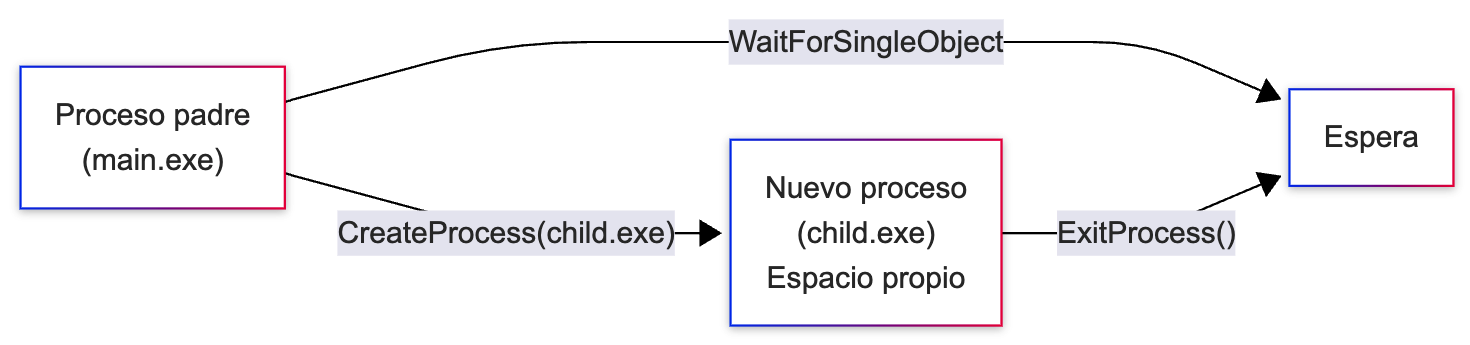
\includegraphics[keepaspectratio,alt={Diagrama de creación de procesos en Windows}]{img/process_creation.png}}
\caption{Diagrama de creación de procesos en Windows}
\end{figure}

\paragraph{\texorpdfstring{Código ---
\texttt{w2\_createprocess.c}}{Código --- w2\_createprocess.c}}\label{cuxf3digo-w2_createprocess.c}

\textbf{Programa hijo (\texttt{w2\_child.c}):}

\begin{Shaded}
\begin{Highlighting}[]
\PreprocessorTok{\#include }\ImportTok{\textless{}stdio.h\textgreater{}}
\PreprocessorTok{\#include }\ImportTok{\textless{}windows.h\textgreater{}}

\DataTypeTok{int}\NormalTok{ main}\OperatorTok{(}\DataTypeTok{void}\OperatorTok{)} \OperatorTok{\{}
\NormalTok{    printf}\OperatorTok{(}\StringTok{"[HIJO]  PID = }\SpecialCharTok{\%lu\textbackslash{}n}\StringTok{"}\OperatorTok{,}\NormalTok{ GetCurrentProcessId}\OperatorTok{());}
\NormalTok{    printf}\OperatorTok{(}\StringTok{"[HIJO]  TID del hilo principal = }\SpecialCharTok{\%lu\textbackslash{}n}\StringTok{"}\OperatorTok{,}\NormalTok{ GetCurrentThreadId}\OperatorTok{());}
\NormalTok{    printf}\OperatorTok{(}\StringTok{"[HIJO]  Ejecutando con argumentos propios...}\SpecialCharTok{\textbackslash{}n}\StringTok{"}\OperatorTok{);}

    \DataTypeTok{int}\NormalTok{ x }\OperatorTok{=} \DecValTok{42}\OperatorTok{;}
    \DataTypeTok{int}\NormalTok{ resultado }\OperatorTok{=}\NormalTok{ x }\OperatorTok{*}\NormalTok{ x}\OperatorTok{;}
\NormalTok{    printf}\OperatorTok{(}\StringTok{"[HIJO]  Cálculo: }\SpecialCharTok{\%d}\StringTok{\^{}2 = }\SpecialCharTok{\%d\textbackslash{}n}\StringTok{"}\OperatorTok{,}\NormalTok{ x}\OperatorTok{,}\NormalTok{ resultado}\OperatorTok{);}

\NormalTok{    printf}\OperatorTok{(}\StringTok{"[HIJO]  Terminando con código 42}\SpecialCharTok{\textbackslash{}n}\StringTok{"}\OperatorTok{);}
    \ControlFlowTok{return} \DecValTok{42}\OperatorTok{;}
\OperatorTok{\}}
\end{Highlighting}
\end{Shaded}

\textbf{Programa padre (\texttt{w2\_createprocess.c}):}

\begin{Shaded}
\begin{Highlighting}[]
\PreprocessorTok{\#include }\ImportTok{\textless{}stdio.h\textgreater{}}
\PreprocessorTok{\#include }\ImportTok{\textless{}windows.h\textgreater{}}

\DataTypeTok{int}\NormalTok{ main}\OperatorTok{(}\DataTypeTok{void}\OperatorTok{)} \OperatorTok{\{}
\NormalTok{    STARTUPINFO si}\OperatorTok{;}
\NormalTok{    PROCESS\_INFORMATION pi}\OperatorTok{;}
\NormalTok{    DWORD codigo\_salida}\OperatorTok{;}

\NormalTok{    ZeroMemory}\OperatorTok{(\&}\NormalTok{si}\OperatorTok{,} \KeywordTok{sizeof}\OperatorTok{(}\NormalTok{si}\OperatorTok{));}
\NormalTok{    si}\OperatorTok{.}\NormalTok{cb }\OperatorTok{=} \KeywordTok{sizeof}\OperatorTok{(}\NormalTok{si}\OperatorTok{);}
\NormalTok{    ZeroMemory}\OperatorTok{(\&}\NormalTok{pi}\OperatorTok{,} \KeywordTok{sizeof}\OperatorTok{(}\NormalTok{pi}\OperatorTok{));}

\NormalTok{    printf}\OperatorTok{(}\StringTok{"[PADRE] PID = }\SpecialCharTok{\%lu}\StringTok{ {-} Creando proceso hijo...}\SpecialCharTok{\textbackslash{}n}\StringTok{"}\OperatorTok{,}
\NormalTok{           GetCurrentProcessId}\OperatorTok{());}

    \ControlFlowTok{if} \OperatorTok{(!}\NormalTok{CreateProcess}\OperatorTok{(}
\NormalTok{            NULL}\OperatorTok{,}            \CommentTok{/* nombre del programa */}
            \StringTok{"w2\_child.exe"}\OperatorTok{,}  \CommentTok{/* línea de comandos */}
\NormalTok{            NULL}\OperatorTok{,}\NormalTok{ NULL}\OperatorTok{,}      \CommentTok{/* seguridad */}
\NormalTok{            FALSE}\OperatorTok{,}           \CommentTok{/* ¿heredar handles? */}
            \DecValTok{0}\OperatorTok{,}               \CommentTok{/* flags de creación */}
\NormalTok{            NULL}\OperatorTok{,}            \CommentTok{/* entorno (hereda el del padre) */}
\NormalTok{            NULL}\OperatorTok{,}            \CommentTok{/* directorio actual (hereda) */}
            \OperatorTok{\&}\NormalTok{si}\OperatorTok{,}             \CommentTok{/* STARTUPINFO */}
            \OperatorTok{\&}\NormalTok{pi}\OperatorTok{))}            \CommentTok{/* PROCESS\_INFORMATION */}
    \OperatorTok{\{}
\NormalTok{        fprintf}\OperatorTok{(}\NormalTok{stderr}\OperatorTok{,} \StringTok{"CreateProcess falló: }\SpecialCharTok{\%lu\textbackslash{}n}\StringTok{"}\OperatorTok{,}\NormalTok{ GetLastError}\OperatorTok{());}
        \ControlFlowTok{return} \DecValTok{1}\OperatorTok{;}
    \OperatorTok{\}}

\NormalTok{    printf}\OperatorTok{(}\StringTok{"[PADRE] Hijo creado: PID = }\SpecialCharTok{\%lu}\StringTok{, TID principal = }\SpecialCharTok{\%lu\textbackslash{}n}\StringTok{"}\OperatorTok{,}
\NormalTok{           pi}\OperatorTok{.}\NormalTok{dwProcessId}\OperatorTok{,}\NormalTok{ pi}\OperatorTok{.}\NormalTok{dwThreadId}\OperatorTok{);}

\NormalTok{    printf}\OperatorTok{(}\StringTok{"[PADRE] Esperando al hijo...}\SpecialCharTok{\textbackslash{}n}\StringTok{"}\OperatorTok{);}
\NormalTok{    WaitForSingleObject}\OperatorTok{(}\NormalTok{pi}\OperatorTok{.}\NormalTok{hProcess}\OperatorTok{,}\NormalTok{ INFINITE}\OperatorTok{);}

\NormalTok{    GetExitCodeProcess}\OperatorTok{(}\NormalTok{pi}\OperatorTok{.}\NormalTok{hProcess}\OperatorTok{,} \OperatorTok{\&}\NormalTok{codigo\_salida}\OperatorTok{);}
\NormalTok{    printf}\OperatorTok{(}\StringTok{"[PADRE] Hijo terminó con código: }\SpecialCharTok{\%lu\textbackslash{}n}\StringTok{"}\OperatorTok{,}\NormalTok{ codigo\_salida}\OperatorTok{);}

\NormalTok{    CloseHandle}\OperatorTok{(}\NormalTok{pi}\OperatorTok{.}\NormalTok{hProcess}\OperatorTok{);}
\NormalTok{    CloseHandle}\OperatorTok{(}\NormalTok{pi}\OperatorTok{.}\NormalTok{hThread}\OperatorTok{);}
\NormalTok{    printf}\OperatorTok{(}\StringTok{"[PADRE] Fin}\SpecialCharTok{\textbackslash{}n}\StringTok{"}\OperatorTok{);}
    \ControlFlowTok{return} \DecValTok{0}\OperatorTok{;}
\OperatorTok{\}}
\end{Highlighting}
\end{Shaded}

\paragraph{Compilación y
ejecución}\label{compilaciuxf3n-y-ejecuciuxf3n-1}

\begin{Shaded}
\begin{Highlighting}[]
\NormalTok{gcc }\AttributeTok{{-}o}\NormalTok{ w2\_child.exe w2\_child.c}
\NormalTok{gcc }\AttributeTok{{-}o}\NormalTok{ w2\_createprocess.exe w2\_createprocess.c}
\NormalTok{w2\_createprocess.exe}
\end{Highlighting}
\end{Shaded}

\paragraph{Verificar independencia de
memoria}\label{verificar-independencia-de-memoria}

Abre una segunda terminal mientras el programa se ejecuta:

\begin{Shaded}
\begin{Highlighting}[]
\FunctionTok{Get{-}Process} \OperatorTok{{-}}\NormalTok{Name w2\_createprocess}\OperatorTok{,}\NormalTok{ w2\_child}
\end{Highlighting}
\end{Shaded}

\paragraph{Salida esperada}\label{salida-esperada-1}

\begin{verbatim}
[PADRE] PID = 24560 - Creando proceso hijo...
[PADRE] Hijo creado: PID = 24588, TID principal = 24589
[PADRE] Esperando al hijo...
[HIJO]  PID = 24588
[HIJO]  TID del hilo principal = 24589
[HIJO]  Ejecutando con argumentos propios...
[HIJO]  Cálculo: 42^2 = 1764
[HIJO]  Terminando con código 42
[PADRE] Hijo terminó con código: 42
[PADRE] Fin
\end{verbatim}

\paragraph{Preguntas de análisis}\label{preguntas-de-anuxe1lisis-1}

\begin{enumerate}
\def\labelenumi{\arabic{enumi}.}
\tightlist
\item
  ¿Qué diferencia fundamental observas entre \texttt{CreateProcess()} de
  Windows y \texttt{fork()} + \texttt{exec()} de UNIX?.
\item
  El hijo se ejecuta en un \textbf{espacio de direcciones separado}. Si
  el hijo modificara una variable global, ¿el padre la vería cambiada?
  ¿Por qué?
\item
  Windows \textbf{no tiene jerarquía de procesos} (árbol). El creador
  recibe un handle. ¿Qué implica esto sobre la relación padre--hijo si
  el padre termina antes que el hijo?
\end{enumerate}

\begin{center}\rule{0.5\linewidth}{0.5pt}\end{center}

\subsection{\texorpdfstring{Ejercicio 2 --- Creación de hilos con
\texttt{CreateThread()}}{Ejercicio 2 --- Creación de hilos con CreateThread()}}\label{ejercicio-2-creaciuxf3n-de-hilos-con-createthread}

\subsubsection{Conceptos relacionados
(Stallings)}\label{conceptos-relacionados-stallings-2}

\texttt{CreateThread()} crea un nuevo \texttt{THREAD\_OBJECT} dentro del
\texttt{PROCESS\_OBJECT} actual. El hilo comparte el espacio de
direcciones, la tabla de handles y los recursos del proceso. Cada hilo
tiene su propia pila, contexto de registros y almacenamiento local
(TLS).

\begin{figure}
\centering
\pandocbounded{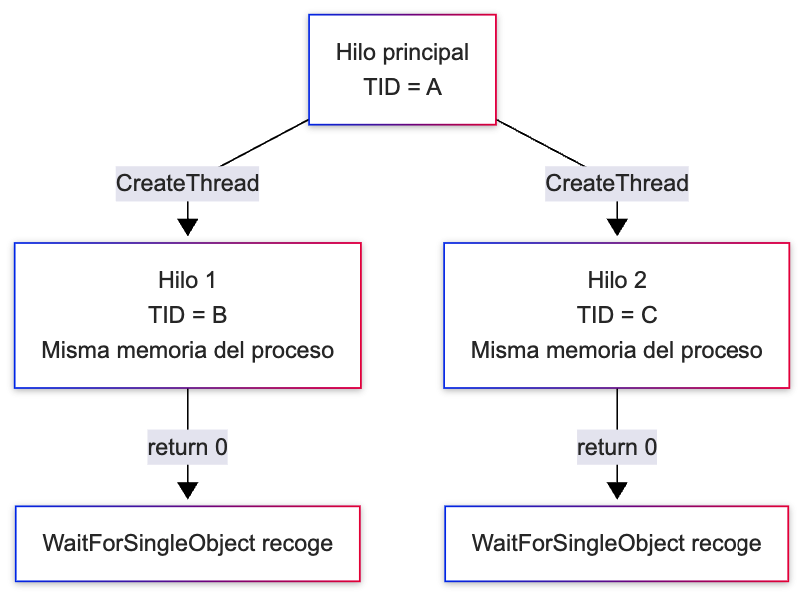
\includegraphics[keepaspectratio,alt={Diagrama de creación de hilos en Windows}]{img/thread_creation.png}}
\caption{Diagrama de creación de hilos en Windows}
\end{figure}

\subsubsection{\texorpdfstring{Código ---
\texttt{w3\_createthread.c}}{Código --- w3\_createthread.c}}\label{cuxf3digo-w3_createthread.c}

\begin{Shaded}
\begin{Highlighting}[]
\PreprocessorTok{\#include }\ImportTok{\textless{}stdio.h\textgreater{}}
\PreprocessorTok{\#include }\ImportTok{\textless{}windows.h\textgreater{}}

\PreprocessorTok{\#define N\_HILOS }\DecValTok{4}

\DataTypeTok{static}\NormalTok{ DWORD WINAPI tarea\_hilo}\OperatorTok{(}\NormalTok{LPVOID lpParam}\OperatorTok{)} \OperatorTok{\{}
    \DataTypeTok{int}\NormalTok{ id }\OperatorTok{=} \OperatorTok{*(}\DataTypeTok{int} \OperatorTok{*)}\NormalTok{lpParam}\OperatorTok{;}

\NormalTok{    printf}\OperatorTok{(}\StringTok{"[hilo }\SpecialCharTok{\%d}\StringTok{] inicio {-} TID = }\SpecialCharTok{\%lu}\StringTok{ (PID = }\SpecialCharTok{\%lu}\StringTok{)}\SpecialCharTok{\textbackslash{}n}\StringTok{"}\OperatorTok{,}
\NormalTok{           id}\OperatorTok{,}\NormalTok{ GetCurrentThreadId}\OperatorTok{(),}\NormalTok{ GetCurrentProcessId}\OperatorTok{());}
    \CommentTok{/* Cada hilo duerme distinto para mostrar concurrencia */}
\NormalTok{    Sleep}\OperatorTok{(}\NormalTok{id }\OperatorTok{*} \DecValTok{500}\OperatorTok{);}
\NormalTok{    printf}\OperatorTok{(}\StringTok{"[hilo }\SpecialCharTok{\%d}\StringTok{] fin}\SpecialCharTok{\textbackslash{}n}\StringTok{"}\OperatorTok{,}\NormalTok{ id}\OperatorTok{);}

    \ControlFlowTok{return}\NormalTok{ id }\OperatorTok{*} \DecValTok{10}\OperatorTok{;}  \CommentTok{/* valor de retorno */}
\OperatorTok{\}}

\DataTypeTok{int}\NormalTok{ main}\OperatorTok{(}\DataTypeTok{void}\OperatorTok{)} \OperatorTok{\{}
\NormalTok{    HANDLE hilos}\OperatorTok{[}\NormalTok{N\_HILOS}\OperatorTok{];}
\NormalTok{    DWORD ids}\OperatorTok{[}\NormalTok{N\_HILOS}\OperatorTok{];}
    \DataTypeTok{int}\NormalTok{ params}\OperatorTok{[}\NormalTok{N\_HILOS}\OperatorTok{];}

\NormalTok{    printf}\OperatorTok{(}\StringTok{"[main] TID = }\SpecialCharTok{\%lu}\StringTok{, PID = }\SpecialCharTok{\%lu\textbackslash{}n}\StringTok{"}\OperatorTok{,}
\NormalTok{           GetCurrentThreadId}\OperatorTok{(),}\NormalTok{ GetCurrentProcessId}\OperatorTok{());}
\NormalTok{    printf}\OperatorTok{(}\StringTok{"[main] Creando }\SpecialCharTok{\%d}\StringTok{ hilos...}\SpecialCharTok{\textbackslash{}n\textbackslash{}n}\StringTok{"}\OperatorTok{,}\NormalTok{ N\_HILOS}\OperatorTok{);}

    \ControlFlowTok{for} \OperatorTok{(}\DataTypeTok{int}\NormalTok{ i }\OperatorTok{=} \DecValTok{0}\OperatorTok{;}\NormalTok{ i }\OperatorTok{\textless{}}\NormalTok{ N\_HILOS}\OperatorTok{;}\NormalTok{ i}\OperatorTok{++)} \OperatorTok{\{}
\NormalTok{        params}\OperatorTok{[}\NormalTok{i}\OperatorTok{]} \OperatorTok{=}\NormalTok{ i }\OperatorTok{+} \DecValTok{1}\OperatorTok{;}
\NormalTok{        hilos}\OperatorTok{[}\NormalTok{i}\OperatorTok{]} \OperatorTok{=}\NormalTok{ CreateThread}\OperatorTok{(}\NormalTok{NULL}\OperatorTok{,} \DecValTok{0}\OperatorTok{,}\NormalTok{ tarea\_hilo}\OperatorTok{,} \OperatorTok{\&}\NormalTok{params}\OperatorTok{[}\NormalTok{i}\OperatorTok{],} \DecValTok{0}\OperatorTok{,} \OperatorTok{\&}\NormalTok{ids}\OperatorTok{[}\NormalTok{i}\OperatorTok{]);}

        \ControlFlowTok{if} \OperatorTok{(}\NormalTok{hilos}\OperatorTok{[}\NormalTok{i}\OperatorTok{]} \OperatorTok{==}\NormalTok{ NULL}\OperatorTok{)} \OperatorTok{\{}
\NormalTok{            fprintf}\OperatorTok{(}\NormalTok{stderr}\OperatorTok{,} \StringTok{"Error creando hilo }\SpecialCharTok{\%d}\StringTok{: }\SpecialCharTok{\%lu\textbackslash{}n}\StringTok{"}\OperatorTok{,}\NormalTok{ i}\OperatorTok{,}\NormalTok{ GetLastError}\OperatorTok{());}
            \ControlFlowTok{return} \DecValTok{1}\OperatorTok{;}
        \OperatorTok{\}}
\NormalTok{        printf}\OperatorTok{(}\StringTok{"[main] Hilo }\SpecialCharTok{\%d}\StringTok{ creado → TID = }\SpecialCharTok{\%lu\textbackslash{}n}\StringTok{"}\OperatorTok{,}\NormalTok{ i }\OperatorTok{+} \DecValTok{1}\OperatorTok{,}\NormalTok{ ids}\OperatorTok{[}\NormalTok{i}\OperatorTok{]);}
    \OperatorTok{\}}

\NormalTok{    printf}\OperatorTok{(}\StringTok{"}\SpecialCharTok{\textbackslash{}n}\StringTok{[main] Esperando a que todos los hilos terminen...}\SpecialCharTok{\textbackslash{}n}\StringTok{"}\OperatorTok{);}

    \CommentTok{/* Esperar a que todos los hilos terminen */}
\NormalTok{    WaitForMultipleObjects}\OperatorTok{(}\NormalTok{N\_HILOS}\OperatorTok{,}\NormalTok{ hilos}\OperatorTok{,}\NormalTok{ TRUE}\OperatorTok{,}\NormalTok{ INFINITE}\OperatorTok{);}

    \CommentTok{/* Recoger valores de retorno */}
    \ControlFlowTok{for} \OperatorTok{(}\DataTypeTok{int}\NormalTok{ i }\OperatorTok{=} \DecValTok{0}\OperatorTok{;}\NormalTok{ i }\OperatorTok{\textless{}}\NormalTok{ N\_HILOS}\OperatorTok{;}\NormalTok{ i}\OperatorTok{++)} \OperatorTok{\{}
\NormalTok{        DWORD retorno}\OperatorTok{;}
\NormalTok{        GetExitCodeThread}\OperatorTok{(}\NormalTok{hilos}\OperatorTok{[}\NormalTok{i}\OperatorTok{],} \OperatorTok{\&}\NormalTok{retorno}\OperatorTok{);}
\NormalTok{        printf}\OperatorTok{(}\StringTok{"[main] Hilo }\SpecialCharTok{\%d}\StringTok{ retornó: }\SpecialCharTok{\%lu\textbackslash{}n}\StringTok{"}\OperatorTok{,}\NormalTok{ i }\OperatorTok{+} \DecValTok{1}\OperatorTok{,}\NormalTok{ retorno}\OperatorTok{);}
\NormalTok{        CloseHandle}\OperatorTok{(}\NormalTok{hilos}\OperatorTok{[}\NormalTok{i}\OperatorTok{]);}
    \OperatorTok{\}}

\NormalTok{    printf}\OperatorTok{(}\StringTok{"}\SpecialCharTok{\textbackslash{}n}\StringTok{[main] Todos los hilos terminaron}\SpecialCharTok{\textbackslash{}n}\StringTok{"}\OperatorTok{);}
    \ControlFlowTok{return} \DecValTok{0}\OperatorTok{;}
\OperatorTok{\}}
\end{Highlighting}
\end{Shaded}

\subsubsection{Compilación y
ejecución}\label{compilaciuxf3n-y-ejecuciuxf3n-2}

\begin{Shaded}
\begin{Highlighting}[]
\NormalTok{gcc }\AttributeTok{{-}o}\NormalTok{ w3\_createthread.exe w3\_createthread.c}
\NormalTok{w3\_createthread.exe}
\end{Highlighting}
\end{Shaded}

\subsubsection{Ver los hilos con Process
Explorer}\label{ver-los-hilos-con-process-explorer}

\begin{enumerate}
\def\labelenumi{\arabic{enumi}.}
\tightlist
\item
  Abre \textbf{Process Explorer} (\texttt{procexp.exe})
\item
  Busca \texttt{w3\_createthread.exe}
\item
  Doble clic → pestaña ``Threads''
\item
  Observa: el hilo principal + 4 hilos, sus TIDs y estados
\end{enumerate}

\subsubsection{Salida esperada}\label{salida-esperada-2}

\begin{verbatim}
[main] TID = 14520, PID = 14520
[main] Creando 4 hilos...

[main] Hilo 1 creado → TID = 15876
[main] Hilo 2 creado → TID = 16132
[main] Hilo 3 creado → TID = 16548
[main] Hilo 4 creado → TID = 16704

[main] Esperando a que todos los hilos terminen...
[hilo 1] inicio - TID = 15876 (PID = 14520)
[hilo 2] inicio - TID = 16132 (PID = 14520)
[hilo 3] inicio - TID = 16548 (PID = 14520)
[hilo 4] inicio - TID = 16704 (PID = 14520)
[hilo 1] fin
[hilo 2] fin
[hilo 3] fin
[hilo 4] fin

[main] Hilo 1 retornó: 10
[main] Hilo 2 retornó: 20
[main] Hilo 3 retornó: 30
[main] Hilo 4 retornó: 40

[main] Todos los hilos terminaron
\end{verbatim}

\subsubsection{Preguntas de análisis}\label{preguntas-de-anuxe1lisis-2}

\begin{enumerate}
\def\labelenumi{\arabic{enumi}.}
\tightlist
\item
  Compara \texttt{CreateThread()} con \texttt{pthread\_create()} del
  laboratorio de Linux. ¿Qué parámetros son equivalentes? ¿Cuál es la
  diferencia en el valor de retorno?
\item
  ¿Por qué los mensajes \texttt{inicio} de los 4 hilos aparecen antes de
  cualquier \texttt{fin}? ¿Qué dice esto sobre la ejecución concurrente?
\item
  ¿Qué representa el \texttt{HANDLE} devuelto por
  \texttt{CreateThread()}?
\end{enumerate}

\begin{center}\rule{0.5\linewidth}{0.5pt}\end{center}

\subsection{Ejercicio 3 --- El ejercicio clave: memoria compartida
(hilos) vs.~separada
(procesos)}\label{ejercicio-3-el-ejercicio-clave-memoria-compartida-hilos-vs.-separada-procesos}

\subsubsection{Conceptos relacionados}\label{conceptos-relacionados}

Este es el ejercicio central del laboratorio. Demuestra
experimentalmente la diferencia fundamental:

{\def\LTcaptype{none} % do not increment counter
\begin{longtable}[]{@{}
  >{\raggedright\arraybackslash}p{(\linewidth - 4\tabcolsep) * \real{0.4848}}
  >{\raggedright\arraybackslash}p{(\linewidth - 4\tabcolsep) * \real{0.3030}}
  >{\raggedright\arraybackslash}p{(\linewidth - 4\tabcolsep) * \real{0.2121}}@{}}
\toprule\noalign{}
\begin{minipage}[b]{\linewidth}\raggedright
Característica
\end{minipage} & \begin{minipage}[b]{\linewidth}\raggedright
Procesos
\end{minipage} & \begin{minipage}[b]{\linewidth}\raggedright
Hilos
\end{minipage} \\
\midrule\noalign{}
\endhead
\bottomrule\noalign{}
\endlastfoot
Espacio de direcciones & \textbf{Separado} --- tabla de páginas propia &
\textbf{Compartido} --- misma tabla de páginas \\
Modificación de variables & Copia privada → cambios no se propagan &
Único valor → cambios visibles entre hilos \\
Aislamiento & Alto & Bajo (riesgo de corrupción) \\
Comunicación & Explícita (IPC) & Directa (variables globales) \\
\end{longtable}
}

\subsubsection{\texorpdfstring{Código ---
\texttt{w4\_compartida.c}}{Código --- w4\_compartida.c}}\label{cuxf3digo-w4_compartida.c}

Este programa se ejecuta a sí mismo como proceso hijo (vía
\texttt{CreateProcess}), demostrando el contraste:

\begin{Shaded}
\begin{Highlighting}[]
\PreprocessorTok{\#include }\ImportTok{\textless{}stdio.h\textgreater{}}
\PreprocessorTok{\#include }\ImportTok{\textless{}string.h\textgreater{}}
\PreprocessorTok{\#include }\ImportTok{\textless{}windows.h\textgreater{}}

\CommentTok{/* Variable global — el centro de la demostración */}
\DataTypeTok{int}\NormalTok{ variable\_compartida }\OperatorTok{=} \DecValTok{0}\OperatorTok{;}

\CommentTok{/* {-}{-}{-}{-} Hilo que modifica la variable {-}{-}{-}{-} */}
\NormalTok{DWORD WINAPI hilo\_modificador}\OperatorTok{(}\NormalTok{LPVOID lpParam}\OperatorTok{)} \OperatorTok{\{}
\NormalTok{    printf}\OperatorTok{(}\StringTok{"  [HILO]  Antes: variable = }\SpecialCharTok{\%d}\StringTok{ (dirección: }\SpecialCharTok{\%p}\StringTok{)}\SpecialCharTok{\textbackslash{}n}\StringTok{"}\OperatorTok{,}
\NormalTok{           variable\_compartida}\OperatorTok{,} \OperatorTok{(}\DataTypeTok{void} \OperatorTok{*)\&}\NormalTok{variable\_compartida}\OperatorTok{);}
\NormalTok{    variable\_compartida }\OperatorTok{=} \DecValTok{777}\OperatorTok{;}
\NormalTok{    printf}\OperatorTok{(}\StringTok{"  [HILO]  Después: variable = }\SpecialCharTok{\%d\textbackslash{}n}\StringTok{"}\OperatorTok{,}\NormalTok{ variable\_compartida}\OperatorTok{);}
    \ControlFlowTok{return} \DecValTok{0}\OperatorTok{;}
\OperatorTok{\}}

\DataTypeTok{int}\NormalTok{ main}\OperatorTok{(}\DataTypeTok{int}\NormalTok{ argc}\OperatorTok{,} \DataTypeTok{char} \OperatorTok{*}\NormalTok{argv}\OperatorTok{[])} \OperatorTok{\{}
    \CommentTok{/* Si se ejecuta con argumento "hijo", actuar como proceso hijo */}
    \ControlFlowTok{if} \OperatorTok{(}\NormalTok{argc }\OperatorTok{\textgreater{}} \DecValTok{1} \OperatorTok{\&\&}\NormalTok{ strcmp}\OperatorTok{(}\NormalTok{argv}\OperatorTok{[}\DecValTok{1}\OperatorTok{],} \StringTok{"hijo"}\OperatorTok{)} \OperatorTok{==} \DecValTok{0}\OperatorTok{)} \OperatorTok{\{}
\NormalTok{        printf}\OperatorTok{(}\StringTok{"  [HIJO PROCESO] Antes: variable = }\SpecialCharTok{\%d}\StringTok{ (dirección: }\SpecialCharTok{\%p}\StringTok{)}\SpecialCharTok{\textbackslash{}n}\StringTok{"}\OperatorTok{,}
\NormalTok{               variable\_compartida}\OperatorTok{,} \OperatorTok{(}\DataTypeTok{void} \OperatorTok{*)\&}\NormalTok{variable\_compartida}\OperatorTok{);}
\NormalTok{        variable\_compartida }\OperatorTok{=} \DecValTok{999}\OperatorTok{;}
\NormalTok{        printf}\OperatorTok{(}\StringTok{"  [HIJO PROCESO] Después: variable = }\SpecialCharTok{\%d\textbackslash{}n}\StringTok{"}\OperatorTok{,}
\NormalTok{               variable\_compartida}\OperatorTok{);}
        \ControlFlowTok{return} \DecValTok{0}\OperatorTok{;}
    \OperatorTok{\}}

    \CommentTok{/* Modo principal */}
\NormalTok{    printf}\OperatorTok{(}\StringTok{"=== DIFERENCIA: HILOS vs PROCESOS en Windows ===}\SpecialCharTok{\textbackslash{}n\textbackslash{}n}\StringTok{"}\OperatorTok{);}
\NormalTok{    printf}\OperatorTok{(}\StringTok{"Valor inicial de variable\_compartida = }\SpecialCharTok{\%d}\StringTok{ (dirección: }\SpecialCharTok{\%p}\StringTok{)}\SpecialCharTok{\textbackslash{}n\textbackslash{}n}\StringTok{"}\OperatorTok{,}
\NormalTok{           variable\_compartida}\OperatorTok{,} \OperatorTok{(}\DataTypeTok{void} \OperatorTok{*)\&}\NormalTok{variable\_compartida}\OperatorTok{);}

    \CommentTok{/* {-}{-}{-} PARTE A: HILO {-}{-}{-} */}
\NormalTok{    printf}\OperatorTok{(}\StringTok{"{-}{-}{-} A) HILO (CreateThread) {-}{-}{-}}\SpecialCharTok{\textbackslash{}n}\StringTok{"}\OperatorTok{);}
\NormalTok{    printf}\OperatorTok{(}\StringTok{"  [MAIN]  Antes = }\SpecialCharTok{\%d\textbackslash{}n}\StringTok{"}\OperatorTok{,}\NormalTok{ variable\_compartida}\OperatorTok{);}

\NormalTok{    HANDLE hilo }\OperatorTok{=}\NormalTok{ CreateThread}\OperatorTok{(}\NormalTok{NULL}\OperatorTok{,} \DecValTok{0}\OperatorTok{,}\NormalTok{ hilo\_modificador}\OperatorTok{,}\NormalTok{ NULL}\OperatorTok{,} \DecValTok{0}\OperatorTok{,}\NormalTok{ NULL}\OperatorTok{);}
\NormalTok{    WaitForSingleObject}\OperatorTok{(}\NormalTok{hilo}\OperatorTok{,}\NormalTok{ INFINITE}\OperatorTok{);}
\NormalTok{    CloseHandle}\OperatorTok{(}\NormalTok{hilo}\OperatorTok{);}

\NormalTok{    printf}\OperatorTok{(}\StringTok{"  [MAIN]  Después = }\SpecialCharTok{\%d}\StringTok{  (el hilo SÍ modificó la variable!)}\SpecialCharTok{\textbackslash{}n\textbackslash{}n}\StringTok{"}\OperatorTok{,}
\NormalTok{           variable\_compartida}\OperatorTok{);}

    \CommentTok{/* {-}{-}{-} PARTE B: PROCESO {-}{-}{-} */}
\NormalTok{    printf}\OperatorTok{(}\StringTok{"{-}{-}{-} B) PROCESO (CreateProcess) {-}{-}{-}}\SpecialCharTok{\textbackslash{}n}\StringTok{"}\OperatorTok{);}
\NormalTok{    printf}\OperatorTok{(}\StringTok{"  [MAIN]  Antes del proceso = }\SpecialCharTok{\%d\textbackslash{}n}\StringTok{"}\OperatorTok{,}\NormalTok{ variable\_compartida}\OperatorTok{);}

\NormalTok{    STARTUPINFO si}\OperatorTok{;}
\NormalTok{    PROCESS\_INFORMATION pi}\OperatorTok{;}
    \DataTypeTok{char}\NormalTok{ cmdline}\OperatorTok{[}\DecValTok{512}\OperatorTok{];}

\NormalTok{    ZeroMemory}\OperatorTok{(\&}\NormalTok{si}\OperatorTok{,} \KeywordTok{sizeof}\OperatorTok{(}\NormalTok{si}\OperatorTok{));}
\NormalTok{    si}\OperatorTok{.}\NormalTok{cb }\OperatorTok{=} \KeywordTok{sizeof}\OperatorTok{(}\NormalTok{si}\OperatorTok{);}
\NormalTok{    ZeroMemory}\OperatorTok{(\&}\NormalTok{pi}\OperatorTok{,} \KeywordTok{sizeof}\OperatorTok{(}\NormalTok{pi}\OperatorTok{));}

    \CommentTok{/* El mismo binario, pero con argumento "hijo" */}
\NormalTok{    GetModuleFileName}\OperatorTok{(}\NormalTok{NULL}\OperatorTok{,}\NormalTok{ cmdline}\OperatorTok{,}\NormalTok{ MAX\_PATH}\OperatorTok{);}
\NormalTok{    strcat}\OperatorTok{(}\NormalTok{cmdline}\OperatorTok{,} \StringTok{" hijo"}\OperatorTok{);}

    \ControlFlowTok{if} \OperatorTok{(!}\NormalTok{CreateProcess}\OperatorTok{(}\NormalTok{NULL}\OperatorTok{,}\NormalTok{ cmdline}\OperatorTok{,}\NormalTok{ NULL}\OperatorTok{,}\NormalTok{ NULL}\OperatorTok{,}\NormalTok{ FALSE}\OperatorTok{,} \DecValTok{0}\OperatorTok{,}
\NormalTok{                       NULL}\OperatorTok{,}\NormalTok{ NULL}\OperatorTok{,} \OperatorTok{\&}\NormalTok{si}\OperatorTok{,} \OperatorTok{\&}\NormalTok{pi}\OperatorTok{))}
    \OperatorTok{\{}
\NormalTok{        fprintf}\OperatorTok{(}\NormalTok{stderr}\OperatorTok{,} \StringTok{"  CreateProcess falló: }\SpecialCharTok{\%lu\textbackslash{}n}\StringTok{"}\OperatorTok{,}\NormalTok{ GetLastError}\OperatorTok{());}
    \OperatorTok{\}} \ControlFlowTok{else} \OperatorTok{\{}
\NormalTok{        WaitForSingleObject}\OperatorTok{(}\NormalTok{pi}\OperatorTok{.}\NormalTok{hProcess}\OperatorTok{,}\NormalTok{ INFINITE}\OperatorTok{);}
\NormalTok{        printf}\OperatorTok{(}\StringTok{"  [MAIN]  Después del proceso = }\SpecialCharTok{\%d}\StringTok{  (NO cambió!)}\SpecialCharTok{\textbackslash{}n}\StringTok{"}\OperatorTok{,}
\NormalTok{               variable\_compartida}\OperatorTok{);}
\NormalTok{        CloseHandle}\OperatorTok{(}\NormalTok{pi}\OperatorTok{.}\NormalTok{hProcess}\OperatorTok{);}
\NormalTok{        CloseHandle}\OperatorTok{(}\NormalTok{pi}\OperatorTok{.}\NormalTok{hThread}\OperatorTok{);}
    \OperatorTok{\}}

\NormalTok{    printf}\OperatorTok{(}\StringTok{"}\SpecialCharTok{\textbackslash{}n}\StringTok{CONCLUSIÓN:}\SpecialCharTok{\textbackslash{}n}\StringTok{"}\OperatorTok{);}
\NormalTok{    printf}\OperatorTok{(}\StringTok{"  CreateThread → el hilo COMPARTE la memoria (variable SÍ cambió)}\SpecialCharTok{\textbackslash{}n}\StringTok{"}\OperatorTok{);}
\NormalTok{    printf}\OperatorTok{(}\StringTok{"  CreateProcess → el proceso tiene su PROPIA COPIA (variable NO cambió)}\SpecialCharTok{\textbackslash{}n}\StringTok{"}\OperatorTok{);}
    \ControlFlowTok{return} \DecValTok{0}\OperatorTok{;}
\OperatorTok{\}}
\end{Highlighting}
\end{Shaded}

\subsubsection{Compilación y
ejecución}\label{compilaciuxf3n-y-ejecuciuxf3n-3}

\begin{Shaded}
\begin{Highlighting}[]
\NormalTok{gcc }\AttributeTok{{-}o}\NormalTok{ w4\_compartida.exe w4\_compartida.c}
\NormalTok{w4\_compartida.exe}
\end{Highlighting}
\end{Shaded}

\subsubsection{Salida esperada}\label{salida-esperada-3}

\begin{verbatim}
=== DIFERENCIA: HILOS vs PROCESOS en Windows ===

Valor inicial de variable_compartida = 0 (dirección: 0x7FF6D3E45010)

--- A) HILO (CreateThread) ---
  [MAIN]  Antes = 0
  [HILO]  Antes: variable = 0 (dirección: 0x7FF6D3E45010)
  [HILO]  Después: variable = 777
  [MAIN]  Después = 777  (el hilo SÍ modificó la variable!)

--- B) PROCESO (CreateProcess) ---
  [MAIN]  Antes del proceso = 777
  [HIJO PROCESO] Antes: variable = 0 (dirección: 0x7FF...)
  [HIJO PROCESO] Después: variable = 999
  [MAIN]  Después del proceso = 777  (NO cambió!)

CONCLUSIÓN:
  CreateThread → el hilo COMPARTE la memoria (variable SÍ cambió)
  CreateProcess → el proceso tiene su PROPIA COPIA (variable NO cambió)
\end{verbatim}

\subsubsection{Preguntas de análisis}\label{preguntas-de-anuxe1lisis-3}

\begin{enumerate}
\def\labelenumi{\arabic{enumi}.}
\tightlist
\item
  El hilo modifica \texttt{variable\_compartida} a 777 y el main
  \textbf{ve} el cambio. El proceso hijo la modifica a 999 y el main
  \textbf{no ve} el cambio. Explica por qué usando el concepto de
  espacio de direcciones virtuales.
\item
  El proceso hijo imprime la misma dirección de memoria virtual que el
  padre. ¿Significa eso que apuntan al mismo marco de página física?
  (Stallings --- memoria virtual vs.~física).
\item
  Según Stallings, ¿cuál es la principal \textbf{ventaja} y la principal
  \textbf{desventaja} de que los hilos compartan memoria?
\end{enumerate}

\begin{center}\rule{0.5\linewidth}{0.5pt}\end{center}

\subsection{Ejercicio 4 --- Estados de hilo en
Windows}\label{ejercicio-4-estados-de-hilo-en-windows}

\subsubsection{Conceptos relacionados}\label{conceptos-relacionados-1}

Windows define \textbf{6 estados} para los hilos, según Stallings:

{\def\LTcaptype{none} % do not increment counter
\begin{longtable}[]{@{}
  >{\raggedright\arraybackslash}p{(\linewidth - 2\tabcolsep) * \real{0.3810}}
  >{\raggedright\arraybackslash}p{(\linewidth - 2\tabcolsep) * \real{0.6190}}@{}}
\toprule\noalign{}
\begin{minipage}[b]{\linewidth}\raggedright
Estado
\end{minipage} & \begin{minipage}[b]{\linewidth}\raggedright
Descripción
\end{minipage} \\
\midrule\noalign{}
\endhead
\bottomrule\noalign{}
\endlastfoot
\textbf{Ready} (Listo) & Puede ser planificado; espera en la cola de
listos \\
\textbf{Standby} (En Espera) & Seleccionado para ejecutar en un
procesador específico \\
\textbf{Running} (Ejecutando) & En ejecución actualmente en un
procesador \\
\textbf{Waiting} (Esperando) & Bloqueado por un evento, E/S,
sincronización o \texttt{Sleep()} \\
\textbf{Transition} (Transición) & Listo para ejecutar pero recursos
(pila) no disponibles \\
\textbf{Terminated} (Terminado) & Finalizó; puede retenerse para
reinicialización \\
\end{longtable}
}

Con \texttt{CreateThread} podemos crear hilos en estado
\textbf{Suspended} (con \texttt{CREATE\_SUSPENDED}) y observar cómo
cambian de estado: Suspended → Ready → Running → Waiting.

\begin{figure}
\centering
\pandocbounded{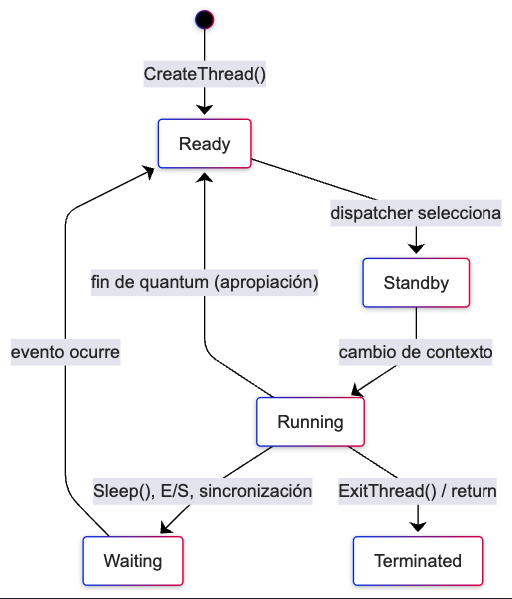
\includegraphics[keepaspectratio,alt={Diagrama de estados de hilo en Windows}]{img/thread_state_machine.png}}
\caption{Diagrama de estados de hilo en Windows}
\end{figure}

\subsubsection{\texorpdfstring{Código ---
\texttt{w5\_estados.c}}{Código --- w5\_estados.c}}\label{cuxf3digo-w5_estados.c}

\begin{Shaded}
\begin{Highlighting}[]
\PreprocessorTok{\#include }\ImportTok{\textless{}stdio.h\textgreater{}}
\PreprocessorTok{\#include }\ImportTok{\textless{}windows.h\textgreater{}}

\CommentTok{/*}
\CommentTok{ * Demostración de los estados de hilo en Windows.}
\CommentTok{ *}
\CommentTok{ * Creamos varios hilos que cambian de estado:}
\CommentTok{ *   Ready → Running → Waiting (Sleep) → Ready → Running → Terminated}
\CommentTok{ *}
\CommentTok{ * Observamos los estados con Process Explorer.}
\CommentTok{ */}

\PreprocessorTok{\#define N\_HILOS }\DecValTok{3}

\DataTypeTok{static}\NormalTok{ DWORD WINAPI hilo\_trabajo}\OperatorTok{(}\NormalTok{LPVOID lpParam}\OperatorTok{)} \OperatorTok{\{}
    \DataTypeTok{int}\NormalTok{ id }\OperatorTok{=} \OperatorTok{*(}\DataTypeTok{int} \OperatorTok{*)}\NormalTok{lpParam}\OperatorTok{;}

\NormalTok{    printf}\OperatorTok{(}\StringTok{"[hilo }\SpecialCharTok{\%d}\StringTok{] INICIO (Running) {-} TID = }\SpecialCharTok{\%lu\textbackslash{}n}\StringTok{"}\OperatorTok{,}
\NormalTok{           id}\OperatorTok{,}\NormalTok{ GetCurrentThreadId}\OperatorTok{());}

    \CommentTok{/* El hilo entra en estado Waiting durante Sleep() */}
\NormalTok{    printf}\OperatorTok{(}\StringTok{"[hilo }\SpecialCharTok{\%d}\StringTok{] Sleeping 3 s (→ Waiting)...}\SpecialCharTok{\textbackslash{}n}\StringTok{"}\OperatorTok{,}\NormalTok{ id}\OperatorTok{);}
\NormalTok{    Sleep}\OperatorTok{(}\DecValTok{3000}\OperatorTok{);}
\NormalTok{    printf}\OperatorTok{(}\StringTok{"[hilo }\SpecialCharTok{\%d}\StringTok{] Desperté (→ Ready → Running)}\SpecialCharTok{\textbackslash{}n}\StringTok{"}\OperatorTok{,}\NormalTok{ id}\OperatorTok{);}

    \CommentTok{/* Simular trabajo en ejecución */}
    \DataTypeTok{volatile} \DataTypeTok{long}\NormalTok{ suma }\OperatorTok{=} \DecValTok{0}\OperatorTok{;}
    \ControlFlowTok{for} \OperatorTok{(}\DataTypeTok{int}\NormalTok{ i }\OperatorTok{=} \DecValTok{0}\OperatorTok{;}\NormalTok{ i }\OperatorTok{\textless{}} \DecValTok{5000000}\OperatorTok{;}\NormalTok{ i}\OperatorTok{++)}
\NormalTok{        suma }\OperatorTok{+=}\NormalTok{ i}\OperatorTok{;}

\NormalTok{    printf}\OperatorTok{(}\StringTok{"[hilo }\SpecialCharTok{\%d}\StringTok{] FIN (→ Terminated), suma = }\SpecialCharTok{\%ld\textbackslash{}n}\StringTok{"}\OperatorTok{,}\NormalTok{ id}\OperatorTok{,}\NormalTok{ suma}\OperatorTok{);}
    \ControlFlowTok{return}\NormalTok{ id }\OperatorTok{*} \DecValTok{100}\OperatorTok{;}
\OperatorTok{\}}

\DataTypeTok{int}\NormalTok{ main}\OperatorTok{(}\DataTypeTok{void}\OperatorTok{)} \OperatorTok{\{}
\NormalTok{    HANDLE hilos}\OperatorTok{[}\NormalTok{N\_HILOS}\OperatorTok{];}
\NormalTok{    DWORD ids}\OperatorTok{[}\NormalTok{N\_HILOS}\OperatorTok{];}
    \DataTypeTok{int}\NormalTok{ params}\OperatorTok{[}\NormalTok{N\_HILOS}\OperatorTok{];}
    \DataTypeTok{int}\NormalTok{ i}\OperatorTok{;}

\NormalTok{    printf}\OperatorTok{(}\StringTok{"=== Estados de Hilo en Windows (Stallings) ===}\SpecialCharTok{\textbackslash{}n\textbackslash{}n}\StringTok{"}\OperatorTok{);}
\NormalTok{    printf}\OperatorTok{(}\StringTok{"Abre Process Explorer y busca este proceso.}\SpecialCharTok{\textbackslash{}n}\StringTok{"}\OperatorTok{);}
\NormalTok{    printf}\OperatorTok{(}\StringTok{"Observa los hilos en la pestaña Threads.}\SpecialCharTok{\textbackslash{}n\textbackslash{}n}\StringTok{"}\OperatorTok{);}

\NormalTok{    printf}\OperatorTok{(}\StringTok{"Creando }\SpecialCharTok{\%d}\StringTok{ hilos en estado SUSPENDIDO...}\SpecialCharTok{\textbackslash{}n}\StringTok{"}\OperatorTok{,}\NormalTok{ N\_HILOS}\OperatorTok{);}
\NormalTok{    printf}\OperatorTok{(}\StringTok{"(Se activarán manualmente)}\SpecialCharTok{\textbackslash{}n\textbackslash{}n}\StringTok{"}\OperatorTok{);}

    \CommentTok{/* Crear hilos en estado SUSPENDIDO para observar Ready → ... */}
    \ControlFlowTok{for} \OperatorTok{(}\NormalTok{i }\OperatorTok{=} \DecValTok{0}\OperatorTok{;}\NormalTok{ i }\OperatorTok{\textless{}}\NormalTok{ N\_HILOS}\OperatorTok{;}\NormalTok{ i}\OperatorTok{++)} \OperatorTok{\{}
\NormalTok{        params}\OperatorTok{[}\NormalTok{i}\OperatorTok{]} \OperatorTok{=}\NormalTok{ i }\OperatorTok{+} \DecValTok{1}\OperatorTok{;}
\NormalTok{        hilos}\OperatorTok{[}\NormalTok{i}\OperatorTok{]} \OperatorTok{=}\NormalTok{ CreateThread}\OperatorTok{(}
\NormalTok{            NULL}\OperatorTok{,}            \CommentTok{/* seguridad */}
            \DecValTok{0}\OperatorTok{,}               \CommentTok{/* pila por defecto */}
\NormalTok{            hilo\_trabajo}\OperatorTok{,}    \CommentTok{/* función */}
            \OperatorTok{\&}\NormalTok{params}\OperatorTok{[}\NormalTok{i}\OperatorTok{],}      \CommentTok{/* parámetro */}
\NormalTok{            CREATE\_SUSPENDED}\OperatorTok{,} \CommentTok{/* ¡crear suspendido! */}
            \OperatorTok{\&}\NormalTok{ids}\OperatorTok{[}\NormalTok{i}\OperatorTok{]);}

        \ControlFlowTok{if} \OperatorTok{(}\NormalTok{hilos}\OperatorTok{[}\NormalTok{i}\OperatorTok{]} \OperatorTok{==}\NormalTok{ NULL}\OperatorTok{)} \OperatorTok{\{}
\NormalTok{            fprintf}\OperatorTok{(}\NormalTok{stderr}\OperatorTok{,} \StringTok{"Error creando hilo }\SpecialCharTok{\%d}\StringTok{: }\SpecialCharTok{\%lu\textbackslash{}n}\StringTok{"}\OperatorTok{,}\NormalTok{ i}\OperatorTok{,}\NormalTok{ GetLastError}\OperatorTok{());}
            \ControlFlowTok{return} \DecValTok{1}\OperatorTok{;}
        \OperatorTok{\}}

\NormalTok{        printf}\OperatorTok{(}\StringTok{"  Hilo }\SpecialCharTok{\%d}\StringTok{ creado (TID = }\SpecialCharTok{\%lu}\StringTok{) {-} estado: SUSPENDED}\SpecialCharTok{\textbackslash{}n}\StringTok{"}\OperatorTok{,}
\NormalTok{               i }\OperatorTok{+} \DecValTok{1}\OperatorTok{,}\NormalTok{ ids}\OperatorTok{[}\NormalTok{i}\OperatorTok{]);}
    \OperatorTok{\}}

\NormalTok{    printf}\OperatorTok{(}\StringTok{"}\SpecialCharTok{\textbackslash{}n}\StringTok{[main] Observa en Process Explorer: los hilos aparecen.}\SpecialCharTok{\textbackslash{}n}\StringTok{"}\OperatorTok{);}
\NormalTok{    printf}\OperatorTok{(}\StringTok{"[main] Presiona Enter para reanudar los hilos...}\SpecialCharTok{\textbackslash{}n}\StringTok{"}\OperatorTok{);}
\NormalTok{    getchar}\OperatorTok{();}

    \CommentTok{/* Reanudar los hilos: Suspended → Ready → Running */}
\NormalTok{    printf}\OperatorTok{(}\StringTok{"[main] Reanudando hilos con ResumeThread()...}\SpecialCharTok{\textbackslash{}n}\StringTok{"}\OperatorTok{);}
    \ControlFlowTok{for} \OperatorTok{(}\NormalTok{i }\OperatorTok{=} \DecValTok{0}\OperatorTok{;}\NormalTok{ i }\OperatorTok{\textless{}}\NormalTok{ N\_HILOS}\OperatorTok{;}\NormalTok{ i}\OperatorTok{++)} \OperatorTok{\{}
\NormalTok{        ResumeThread}\OperatorTok{(}\NormalTok{hilos}\OperatorTok{[}\NormalTok{i}\OperatorTok{]);}
\NormalTok{        printf}\OperatorTok{(}\StringTok{"  Hilo }\SpecialCharTok{\%d}\StringTok{ reanudado (TID = }\SpecialCharTok{\%lu}\StringTok{)}\SpecialCharTok{\textbackslash{}n}\StringTok{"}\OperatorTok{,}\NormalTok{ i }\OperatorTok{+} \DecValTok{1}\OperatorTok{,}\NormalTok{ ids}\OperatorTok{[}\NormalTok{i}\OperatorTok{]);}
    \OperatorTok{\}}

\NormalTok{    printf}\OperatorTok{(}\StringTok{"}\SpecialCharTok{\textbackslash{}n}\StringTok{[main] Esperando a que terminen...}\SpecialCharTok{\textbackslash{}n}\StringTok{"}\OperatorTok{);}
\NormalTok{    WaitForMultipleObjects}\OperatorTok{(}\NormalTok{N\_HILOS}\OperatorTok{,}\NormalTok{ hilos}\OperatorTok{,}\NormalTok{ TRUE}\OperatorTok{,}\NormalTok{ INFINITE}\OperatorTok{);}

    \ControlFlowTok{for} \OperatorTok{(}\NormalTok{i }\OperatorTok{=} \DecValTok{0}\OperatorTok{;}\NormalTok{ i }\OperatorTok{\textless{}}\NormalTok{ N\_HILOS}\OperatorTok{;}\NormalTok{ i}\OperatorTok{++)} \OperatorTok{\{}
\NormalTok{        DWORD retorno}\OperatorTok{;}
\NormalTok{        GetExitCodeThread}\OperatorTok{(}\NormalTok{hilos}\OperatorTok{[}\NormalTok{i}\OperatorTok{],} \OperatorTok{\&}\NormalTok{retorno}\OperatorTok{);}
\NormalTok{        printf}\OperatorTok{(}\StringTok{"  Hilo }\SpecialCharTok{\%d}\StringTok{ → retorno = }\SpecialCharTok{\%lu\textbackslash{}n}\StringTok{"}\OperatorTok{,}\NormalTok{ i }\OperatorTok{+} \DecValTok{1}\OperatorTok{,}\NormalTok{ retorno}\OperatorTok{);}
\NormalTok{        CloseHandle}\OperatorTok{(}\NormalTok{hilos}\OperatorTok{[}\NormalTok{i}\OperatorTok{]);}
    \OperatorTok{\}}

\NormalTok{    printf}\OperatorTok{(}\StringTok{"}\SpecialCharTok{\textbackslash{}n}\StringTok{[main] Todos los hilos terminaron.}\SpecialCharTok{\textbackslash{}n}\StringTok{"}\OperatorTok{);}
\NormalTok{    printf}\OperatorTok{(}\StringTok{"}\SpecialCharTok{\textbackslash{}n}\StringTok{Estados observados:}\SpecialCharTok{\textbackslash{}n}\StringTok{"}\OperatorTok{);}
\NormalTok{    printf}\OperatorTok{(}\StringTok{"  CreateThread(CREATE\_SUSPENDED) → SUSPENDED}\SpecialCharTok{\textbackslash{}n}\StringTok{"}\OperatorTok{);}
\NormalTok{    printf}\OperatorTok{(}\StringTok{"  ResumeThread() → Ready → Running}\SpecialCharTok{\textbackslash{}n}\StringTok{"}\OperatorTok{);}
\NormalTok{    printf}\OperatorTok{(}\StringTok{"  Sleep()       → Waiting → Ready → Running}\SpecialCharTok{\textbackslash{}n}\StringTok{"}\OperatorTok{);}
\NormalTok{    printf}\OperatorTok{(}\StringTok{"  return        → Terminated}\SpecialCharTok{\textbackslash{}n}\StringTok{"}\OperatorTok{);}
    \ControlFlowTok{return} \DecValTok{0}\OperatorTok{;}
\OperatorTok{\}}
\end{Highlighting}
\end{Shaded}

\subsubsection{Compilación y
ejecución}\label{compilaciuxf3n-y-ejecuciuxf3n-4}

\begin{Shaded}
\begin{Highlighting}[]
\NormalTok{gcc }\AttributeTok{{-}o}\NormalTok{ w5\_estados.exe w5\_estados.c}
\NormalTok{w5\_estados.exe}
\end{Highlighting}
\end{Shaded}

\subsubsection{Observación con Process
Explorer}\label{observaciuxf3n-con-process-explorer}

\begin{enumerate}
\def\labelenumi{\arabic{enumi}.}
\tightlist
\item
  Abre \textbf{Process Explorer}
\item
  Cuando el programa muestre ``Presiona Enter\ldots{}'', busca el
  proceso en la lista
\item
  Doble clic → pestaña ``Threads''
\item
  Verás los 3 hilos en estado \textbf{Suspended} (o similares)
\item
  Presiona Enter en el programa y observa los cambios de estado
\item
  Durante el \texttt{Sleep(3000)}, los hilos aparecerán en estado
  \textbf{Waiting}
\end{enumerate}

\subsubsection{Salida esperada}\label{salida-esperada-4}

\begin{verbatim}
=== Estados de Hilo en Windows (Stallings) ===

Abre Process Explorer y busca este proceso.
Observa los hilos en la pestaña Threads.

Creando 3 hilos en estado SUSPENDIDO...
(Se activarán manualmente)

  Hilo 1 creado (TID = 18240) - estado: SUSPENDED
  Hilo 2 creado (TID = 18276) - estado: SUSPENDED
  Hilo 3 creado (TID = 18312) - estado: SUSPENDED

[main] Observa en Process Explorer: los hilos aparecen.
[main] Presiona Enter para reanudar los hilos...

[main] Reanudando hilos con ResumeThread()...
  Hilo 1 reanudado (TID = 18240)
  Hilo 2 reanudado (TID = 18276)
  Hilo 3 reanudado (TID = 18312)

[main] Esperando a que terminen...
[hilo 1] INICIO (Running) - TID = 18240
[hilo 2] INICIO (Running) - TID = 18276
[hilo 3] INICIO (Running) - TID = 18312
[hilo 1] Sleeping 3 s (→ Waiting)...
[hilo 2] Sleeping 3 s (→ Waiting)...
[hilo 3] Sleeping 3 s (→ Waiting)...
[hilo 1] Desperté (→ Ready → Running)
[hilo 2] Desperté (→ Ready → Running)
[hilo 3] Desperté (→ Ready → Running)
[hilo 1] FIN (→ Terminated), suma = ...
[hilo 2] FIN (→ Terminated), suma = ...
[hilo 3] FIN (→ Terminated), suma = ...

  Hilo 1 → retorno = 100
  Hilo 2 → retorno = 200
  Hilo 3 → retorno = 300

[main] Todos los hilos terminaron.

Estados observados:
  CreateThread(CREATE_SUSPENDED) → SUSPENDED
  ResumeThread() → Ready → Running
  Sleep()       → Waiting → Ready → Running
  return        → Terminated
\end{verbatim}

\subsubsection{Preguntas de análisis}\label{preguntas-de-anuxe1lisis-4}

\begin{enumerate}
\def\labelenumi{\arabic{enumi}.}
\tightlist
\item
  Según Stallings, Windows tiene 6 estados de hilo. ¿Cuáles observaste
  directamente en este ejercicio? ¿Cuáles no?
\item
  ¿Qué diferencia hay entre \textbf{Ready} y \textbf{Standby} en
  Windows? (Pista: Standby es un estado de transición muy breve).
\end{enumerate}

\begin{center}\rule{0.5\linewidth}{0.5pt}\end{center}

\subsection{Ejercicio 5 --- Objeto Proceso vs.~Objeto Hilo en
Windows}\label{ejercicio-5-objeto-proceso-vs.-objeto-hilo-en-windows}

\subsubsection{Conceptos relacionados}\label{conceptos-relacionados-2}

Stallings explica que Windows distingue explícitamente entre:

\begin{itemize}
\tightlist
\item
  \textbf{\texttt{PROCESS\_OBJECT}}: tiene espacio de direcciones, tabla
  de handles, descriptores de seguridad, prioridad base, afinidad de
  procesador, límites de cuota
\item
  \textbf{\texttt{THREAD\_OBJECT}}: tiene contexto de registros,
  prioridad dinámica, contador de suspensión, estado de alerta, token de
  suplantación
\end{itemize}

Un proceso Windows \textbf{no puede ejecutar sin un hilo}.
\texttt{CreateProcess()} siempre crea el proceso \textbf{y} su hilo
principal automáticamente. \texttt{CreateThread()} solo crea hilos
adicionales dentro de un proceso existente.

\begin{figure}
\centering
\pandocbounded{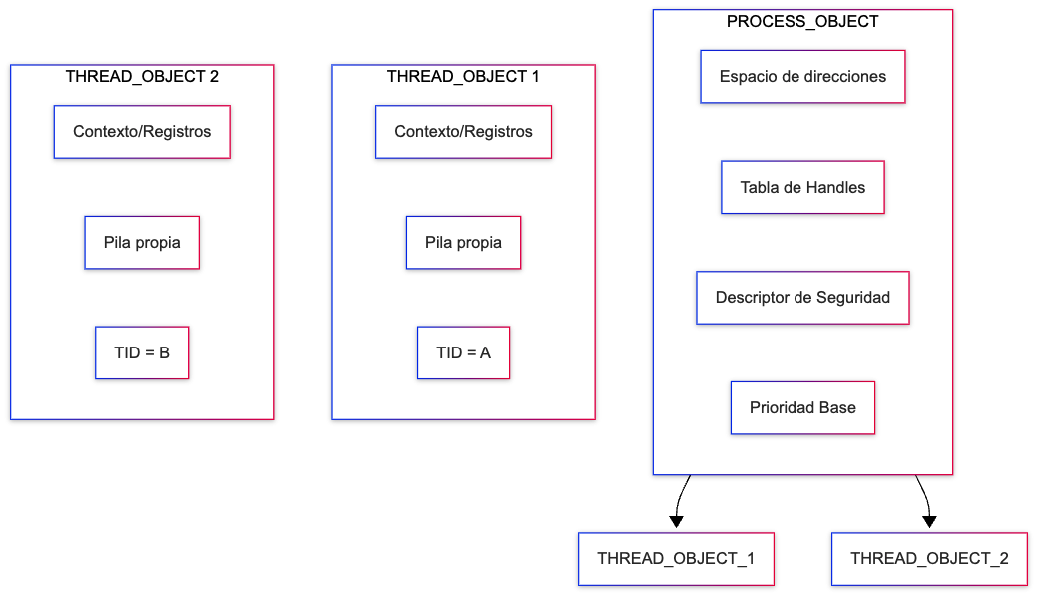
\includegraphics[keepaspectratio,alt={Proceso vs Hilo}]{img/process_thread_management.png}}
\caption{Proceso vs Hilo}
\end{figure}

Este ejercicio crea un proceso y explora la relación proceso ↔ hilos
centralizada en el \textbf{PROCESS\_INFORMATION}.

\subsubsection{\texorpdfstring{Código ---
\texttt{w6\_objetos.c}}{Código --- w6\_objetos.c}}\label{cuxf3digo-w6_objetos.c}

\begin{Shaded}
\begin{Highlighting}[]
\PreprocessorTok{\#include }\ImportTok{\textless{}stdio.h\textgreater{}}
\PreprocessorTok{\#include }\ImportTok{\textless{}windows.h\textgreater{}}

\CommentTok{/*}
\CommentTok{ * Stallings: PROCESS\_OBJECT vs THREAD\_OBJECT}
\CommentTok{ *}
\CommentTok{ * Demostración de que:}
\CommentTok{ * 1. CreateProcess() crea un proceso + su hilo principal}
\CommentTok{ * 2. CreateThread() crea hilos adicionales dentro del proceso}
\CommentTok{ * 3. Cada hilo tiene su propio TID (THREAD\_OBJECT)}
\CommentTok{ * 4. El proceso tiene un PID (PROCESS\_OBJECT)}
\CommentTok{ *}
\CommentTok{ * El programa se ejecuta a sí mismo como hijo.}
\CommentTok{ */}

\DataTypeTok{static}\NormalTok{ DWORD WINAPI hilo\_padre}\OperatorTok{(}\NormalTok{LPVOID lpParam}\OperatorTok{);}
\DataTypeTok{static}\NormalTok{ DWORD WINAPI hilo\_hijo}\OperatorTok{(}\NormalTok{LPVOID lpParam}\OperatorTok{);}

\DataTypeTok{int}\NormalTok{ main}\OperatorTok{(}\DataTypeTok{int}\NormalTok{ argc}\OperatorTok{,} \DataTypeTok{char} \OperatorTok{*}\NormalTok{argv}\OperatorTok{[])} \OperatorTok{\{}
    \CommentTok{/* Modo hijo */}
    \ControlFlowTok{if} \OperatorTok{(}\NormalTok{argc }\OperatorTok{\textgreater{}} \DecValTok{1} \OperatorTok{\&\&}\NormalTok{ strcmp}\OperatorTok{(}\NormalTok{argv}\OperatorTok{[}\DecValTok{1}\OperatorTok{],} \StringTok{"child"}\OperatorTok{)} \OperatorTok{==} \DecValTok{0}\OperatorTok{)} \OperatorTok{\{}
\NormalTok{        printf}\OperatorTok{(}\StringTok{"[HIJO]  PID (PROCESS\_OBJECT) = }\SpecialCharTok{\%lu\textbackslash{}n}\StringTok{"}\OperatorTok{,}\NormalTok{ GetCurrentProcessId}\OperatorTok{());}
\NormalTok{        printf}\OperatorTok{(}\StringTok{"[HIJO]  TID (THREAD\_OBJECT)  = }\SpecialCharTok{\%lu\textbackslash{}n}\StringTok{"}\OperatorTok{,}\NormalTok{ GetCurrentThreadId}\OperatorTok{());}

        \CommentTok{/* El hijo crea 2 hilos adicionales */}
\NormalTok{        printf}\OperatorTok{(}\StringTok{"[HIJO]  Creando 2 hilos propios...}\SpecialCharTok{\textbackslash{}n}\StringTok{"}\OperatorTok{);}

\NormalTok{        HANDLE h\_hijo}\OperatorTok{[}\DecValTok{2}\OperatorTok{];}
\NormalTok{        DWORD id\_h}\OperatorTok{[}\DecValTok{2}\OperatorTok{];}

        \ControlFlowTok{for} \OperatorTok{(}\DataTypeTok{int}\NormalTok{ i }\OperatorTok{=} \DecValTok{0}\OperatorTok{;}\NormalTok{ i }\OperatorTok{\textless{}} \DecValTok{2}\OperatorTok{;}\NormalTok{ i}\OperatorTok{++)} \OperatorTok{\{}
\NormalTok{            h\_hijo}\OperatorTok{[}\NormalTok{i}\OperatorTok{]} \OperatorTok{=}\NormalTok{ CreateThread}\OperatorTok{(}\NormalTok{NULL}\OperatorTok{,} \DecValTok{0}\OperatorTok{,}
                \OperatorTok{(}\NormalTok{LPTHREAD\_START\_ROUTINE}\OperatorTok{)}\NormalTok{hilo\_hijo}\OperatorTok{,}\NormalTok{ NULL}\OperatorTok{,} \DecValTok{0}\OperatorTok{,} \OperatorTok{\&}\NormalTok{id\_h}\OperatorTok{[}\NormalTok{i}\OperatorTok{]);}
\NormalTok{            printf}\OperatorTok{(}\StringTok{"[HIJO]  Nuevo THREAD\_OBJECT }\SpecialCharTok{\%d}\StringTok{ → TID = }\SpecialCharTok{\%lu\textbackslash{}n}\StringTok{"}\OperatorTok{,}
\NormalTok{                   i }\OperatorTok{+} \DecValTok{1}\OperatorTok{,}\NormalTok{ id\_h}\OperatorTok{[}\NormalTok{i}\OperatorTok{]);}
        \OperatorTok{\}}

\NormalTok{        WaitForMultipleObjects}\OperatorTok{(}\DecValTok{2}\OperatorTok{,}\NormalTok{ h\_hijo}\OperatorTok{,}\NormalTok{ TRUE}\OperatorTok{,}\NormalTok{ INFINITE}\OperatorTok{);}
        \ControlFlowTok{for} \OperatorTok{(}\DataTypeTok{int}\NormalTok{ i }\OperatorTok{=} \DecValTok{0}\OperatorTok{;}\NormalTok{ i }\OperatorTok{\textless{}} \DecValTok{2}\OperatorTok{;}\NormalTok{ i}\OperatorTok{++)}\NormalTok{ CloseHandle}\OperatorTok{(}\NormalTok{h\_hijo}\OperatorTok{[}\NormalTok{i}\OperatorTok{]);}

\NormalTok{        printf}\OperatorTok{(}\StringTok{"[HIJO]  Terminando {-} el PROCESS\_OBJECT y sus 3 THREAD\_OBJECT}\SpecialCharTok{\textbackslash{}n}\StringTok{"}\OperatorTok{);}
        \ControlFlowTok{return} \DecValTok{42}\OperatorTok{;}
    \OperatorTok{\}}

    \CommentTok{/* {-}{-}{-}{-} PADRE {-}{-}{-}{-} */}
\NormalTok{    DWORD pid\_actual }\OperatorTok{=}\NormalTok{ GetCurrentProcessId}\OperatorTok{();}
\NormalTok{    DWORD tid\_actual }\OperatorTok{=}\NormalTok{ GetCurrentThreadId}\OperatorTok{();}

\NormalTok{    printf}\OperatorTok{(}\StringTok{"=== Stallings: PROCESS\_OBJECT vs THREAD\_OBJECT ===}\SpecialCharTok{\textbackslash{}n\textbackslash{}n}\StringTok{"}\OperatorTok{);}
\NormalTok{    printf}\OperatorTok{(}\StringTok{"[PADRE] Este PROCESO (PROCESS\_OBJECT): PID = }\SpecialCharTok{\%lu\textbackslash{}n}\StringTok{"}\OperatorTok{,}\NormalTok{ pid\_actual}\OperatorTok{);}
\NormalTok{    printf}\OperatorTok{(}\StringTok{"[PADRE]   Hilo principal (THREAD\_OBJECT): TID = }\SpecialCharTok{\%lu\textbackslash{}n}\StringTok{"}\OperatorTok{,}\NormalTok{ tid\_actual}\OperatorTok{);}

    \CommentTok{/* Crear 2 hilos en el padre */}
\NormalTok{    printf}\OperatorTok{(}\StringTok{"[PADRE] Creando 2 hilos adicionales en el MISMO proceso...}\SpecialCharTok{\textbackslash{}n}\StringTok{"}\OperatorTok{);}

\NormalTok{    HANDLE h\_padre}\OperatorTok{[}\DecValTok{2}\OperatorTok{];}
\NormalTok{    DWORD ids\_adicionales}\OperatorTok{[}\DecValTok{2}\OperatorTok{];}

\NormalTok{    printf}\OperatorTok{(}\StringTok{"[PADRE]   THREAD\_OBJECT adicionales creados:}\SpecialCharTok{\textbackslash{}n}\StringTok{"}\OperatorTok{);}
    \ControlFlowTok{for} \OperatorTok{(}\DataTypeTok{int}\NormalTok{ i }\OperatorTok{=} \DecValTok{0}\OperatorTok{;}\NormalTok{ i }\OperatorTok{\textless{}} \DecValTok{2}\OperatorTok{;}\NormalTok{ i}\OperatorTok{++)} \OperatorTok{\{}
\NormalTok{        h\_padre}\OperatorTok{[}\NormalTok{i}\OperatorTok{]} \OperatorTok{=}\NormalTok{ CreateThread}\OperatorTok{(}\NormalTok{NULL}\OperatorTok{,} \DecValTok{0}\OperatorTok{,}
            \OperatorTok{(}\NormalTok{LPTHREAD\_START\_ROUTINE}\OperatorTok{)}\NormalTok{hilo\_padre}\OperatorTok{,}\NormalTok{ NULL}\OperatorTok{,} \DecValTok{0}\OperatorTok{,} \OperatorTok{\&}\NormalTok{ids\_adicionales}\OperatorTok{[}\NormalTok{i}\OperatorTok{]);}
\NormalTok{        printf}\OperatorTok{(}\StringTok{"[PADRE]     Hilo }\SpecialCharTok{\%d}\StringTok{ → TID = }\SpecialCharTok{\%lu\textbackslash{}n}\StringTok{"}\OperatorTok{,}\NormalTok{ i }\OperatorTok{+} \DecValTok{1}\OperatorTok{,}\NormalTok{ ids\_adicionales}\OperatorTok{[}\NormalTok{i}\OperatorTok{]);}
    \OperatorTok{\}}
\NormalTok{    WaitForMultipleObjects}\OperatorTok{(}\DecValTok{2}\OperatorTok{,}\NormalTok{ h\_padre}\OperatorTok{,}\NormalTok{ TRUE}\OperatorTok{,}\NormalTok{ INFINITE}\OperatorTok{);}
    \ControlFlowTok{for} \OperatorTok{(}\DataTypeTok{int}\NormalTok{ i }\OperatorTok{=} \DecValTok{0}\OperatorTok{;}\NormalTok{ i }\OperatorTok{\textless{}} \DecValTok{2}\OperatorTok{;}\NormalTok{ i}\OperatorTok{++)}\NormalTok{ CloseHandle}\OperatorTok{(}\NormalTok{h\_padre}\OperatorTok{[}\NormalTok{i}\OperatorTok{]);}

\NormalTok{    printf}\OperatorTok{(}\StringTok{"}\SpecialCharTok{\textbackslash{}n}\StringTok{[PADRE] Ahora: }\SpecialCharTok{\%d}\StringTok{ THREAD\_OBJECT vivos en este proceso}\SpecialCharTok{\textbackslash{}n}\StringTok{"}\OperatorTok{,} \DecValTok{1} \OperatorTok{+} \DecValTok{2}\OperatorTok{);}

    \CommentTok{/* Crear un PROCESO HIJO con CreateProcess */}
\NormalTok{    printf}\OperatorTok{(}\StringTok{"}\SpecialCharTok{\textbackslash{}n}\StringTok{[PADRE] Creando un NUEVO PROCESO (CreateProcess)...}\SpecialCharTok{\textbackslash{}n}\StringTok{"}\OperatorTok{);}

\NormalTok{    STARTUPINFO si}\OperatorTok{;}
\NormalTok{    PROCESS\_INFORMATION pi}\OperatorTok{;}
    \DataTypeTok{char}\NormalTok{ cmdline}\OperatorTok{[}\DecValTok{512}\OperatorTok{];}
\NormalTok{    ZeroMemory}\OperatorTok{(\&}\NormalTok{si}\OperatorTok{,} \KeywordTok{sizeof}\OperatorTok{(}\NormalTok{si}\OperatorTok{));}
\NormalTok{    si}\OperatorTok{.}\NormalTok{cb }\OperatorTok{=} \KeywordTok{sizeof}\OperatorTok{(}\NormalTok{si}\OperatorTok{);}
\NormalTok{    ZeroMemory}\OperatorTok{(\&}\NormalTok{pi}\OperatorTok{,} \KeywordTok{sizeof}\OperatorTok{(}\NormalTok{pi}\OperatorTok{));}

\NormalTok{    GetModuleFileName}\OperatorTok{(}\NormalTok{NULL}\OperatorTok{,}\NormalTok{ cmdline}\OperatorTok{,}\NormalTok{ MAX\_PATH}\OperatorTok{);}
\NormalTok{    strcat}\OperatorTok{(}\NormalTok{cmdline}\OperatorTok{,} \StringTok{" child"}\OperatorTok{);}

    \ControlFlowTok{if} \OperatorTok{(!}\NormalTok{CreateProcess}\OperatorTok{(}\NormalTok{NULL}\OperatorTok{,}\NormalTok{ cmdline}\OperatorTok{,}\NormalTok{ NULL}\OperatorTok{,}\NormalTok{ NULL}\OperatorTok{,}\NormalTok{ FALSE}\OperatorTok{,} \DecValTok{0}\OperatorTok{,}
\NormalTok{                       NULL}\OperatorTok{,}\NormalTok{ NULL}\OperatorTok{,} \OperatorTok{\&}\NormalTok{si}\OperatorTok{,} \OperatorTok{\&}\NormalTok{pi}\OperatorTok{))}
    \OperatorTok{\{}
\NormalTok{        fprintf}\OperatorTok{(}\NormalTok{stderr}\OperatorTok{,} \StringTok{"CreateProcess falló: }\SpecialCharTok{\%lu\textbackslash{}n}\StringTok{"}\OperatorTok{,}\NormalTok{ GetLastError}\OperatorTok{());}
        \ControlFlowTok{return} \DecValTok{1}\OperatorTok{;}
    \OperatorTok{\}}

\NormalTok{    printf}\OperatorTok{(}\StringTok{"[PADRE] Nuevo PROCESS\_OBJECT creado:}\SpecialCharTok{\textbackslash{}n}\StringTok{"}\OperatorTok{);}
\NormalTok{    printf}\OperatorTok{(}\StringTok{"[PADRE]   PID del hijo = }\SpecialCharTok{\%lu\textbackslash{}n}\StringTok{"}\OperatorTok{,}\NormalTok{ pi}\OperatorTok{.}\NormalTok{dwProcessId}\OperatorTok{);}
\NormalTok{    printf}\OperatorTok{(}\StringTok{"[PADRE]   TID del hilo principal del hijo = }\SpecialCharTok{\%lu\textbackslash{}n}\StringTok{"}\OperatorTok{,}\NormalTok{ pi}\OperatorTok{.}\NormalTok{dwThreadId}\OperatorTok{);}

\NormalTok{    WaitForSingleObject}\OperatorTok{(}\NormalTok{pi}\OperatorTok{.}\NormalTok{hProcess}\OperatorTok{,}\NormalTok{ INFINITE}\OperatorTok{);}

\NormalTok{    DWORD codigo}\OperatorTok{;}
\NormalTok{    GetExitCodeProcess}\OperatorTok{(}\NormalTok{pi}\OperatorTok{.}\NormalTok{hProcess}\OperatorTok{,} \OperatorTok{\&}\NormalTok{codigo}\OperatorTok{);}
\NormalTok{    printf}\OperatorTok{(}\StringTok{"[PADRE] Hijo terminó con código: }\SpecialCharTok{\%lu\textbackslash{}n}\StringTok{"}\OperatorTok{,}\NormalTok{ codigo}\OperatorTok{);}

\NormalTok{    CloseHandle}\OperatorTok{(}\NormalTok{pi}\OperatorTok{.}\NormalTok{hProcess}\OperatorTok{);}
\NormalTok{    CloseHandle}\OperatorTok{(}\NormalTok{pi}\OperatorTok{.}\NormalTok{hThread}\OperatorTok{);}

\NormalTok{    printf}\OperatorTok{(}\StringTok{"}\SpecialCharTok{\textbackslash{}n}\StringTok{RESUMEN:}\SpecialCharTok{\textbackslash{}n}\StringTok{"}\OperatorTok{);}
\NormalTok{    printf}\OperatorTok{(}\StringTok{"  PROCESS\_OBJECT (}\SpecialCharTok{\%lu}\StringTok{): contiene THREAD\_OBJECTs}\SpecialCharTok{\textbackslash{}n}\StringTok{"}\OperatorTok{,}\NormalTok{ pid\_actual}\OperatorTok{);}
\NormalTok{    printf}\OperatorTok{(}\StringTok{"    {-} Hilo principal: TID = }\SpecialCharTok{\%lu\textbackslash{}n}\StringTok{"}\OperatorTok{,}\NormalTok{ tid\_actual}\OperatorTok{);}
\NormalTok{    printf}\OperatorTok{(}\StringTok{"    {-} Hilos adicionales: }\SpecialCharTok{\%lu}\StringTok{, }\SpecialCharTok{\%lu\textbackslash{}n}\StringTok{"}\OperatorTok{,}
\NormalTok{           ids\_adicionales}\OperatorTok{[}\DecValTok{0}\OperatorTok{],}\NormalTok{ ids\_adicionales}\OperatorTok{[}\DecValTok{1}\OperatorTok{]);}
\NormalTok{    printf}\OperatorTok{(}\StringTok{"  PROCESS\_OBJECT hijo (}\SpecialCharTok{\%lu}\StringTok{): creado con CreateProcess()}\SpecialCharTok{\textbackslash{}n}\StringTok{"}\OperatorTok{,}
\NormalTok{           pi}\OperatorTok{.}\NormalTok{dwProcessId}\OperatorTok{);}
\NormalTok{    printf}\OperatorTok{(}\StringTok{"    {-} Trae su primer THREAD\_OBJECT automáticamente (TID = }\SpecialCharTok{\%lu}\StringTok{)}\SpecialCharTok{\textbackslash{}n}\StringTok{"}\OperatorTok{,}
\NormalTok{           pi}\OperatorTok{.}\NormalTok{dwThreadId}\OperatorTok{);}
\NormalTok{    printf}\OperatorTok{(}\StringTok{"  Cada THREAD\_OBJECT tiene: pila propia, contexto, prioridad}\SpecialCharTok{\textbackslash{}n}\StringTok{"}\OperatorTok{);}
\NormalTok{    printf}\OperatorTok{(}\StringTok{"  Cada PROCESS\_OBJECT tiene: espacio dir., handles, cuotas}\SpecialCharTok{\textbackslash{}n}\StringTok{"}\OperatorTok{);}
    \ControlFlowTok{return} \DecValTok{0}\OperatorTok{;}
\OperatorTok{\}}

\CommentTok{/* Función para hilos del padre */}
\DataTypeTok{static}\NormalTok{ DWORD WINAPI hilo\_padre}\OperatorTok{(}\NormalTok{LPVOID lpParam}\OperatorTok{)} \OperatorTok{\{}
\NormalTok{    Sleep}\OperatorTok{(}\DecValTok{100}\OperatorTok{);}
    \ControlFlowTok{return} \DecValTok{0}\OperatorTok{;}
\OperatorTok{\}}

\CommentTok{/* Función para hilos del hijo */}
\DataTypeTok{static}\NormalTok{ DWORD WINAPI hilo\_hijo}\OperatorTok{(}\NormalTok{LPVOID lpParam}\OperatorTok{)} \OperatorTok{\{}
\NormalTok{    Sleep}\OperatorTok{(}\DecValTok{100}\OperatorTok{);}
    \ControlFlowTok{return} \DecValTok{0}\OperatorTok{;}
\OperatorTok{\}}
\end{Highlighting}
\end{Shaded}

\begin{quote}
\textbf{Nota de compilación:} \texttt{hilo\_padre} e \texttt{hilo\_hijo}
se usan como argumentos de \texttt{CreateThread()} antes de su
definición al final del archivo, por lo que necesitan las declaraciones
adelantadas (\texttt{static\ DWORD\ WINAPI\ hilo\_padre(LPVOID);} etc.)
mostradas arriba. Sin ellas, \texttt{gcc} falla con
\texttt{error:\ \textquotesingle{}hilo\_hijo\textquotesingle{}\ undeclared}.
\end{quote}

\subsubsection{Compilación y
ejecución}\label{compilaciuxf3n-y-ejecuciuxf3n-5}

\begin{Shaded}
\begin{Highlighting}[]
\NormalTok{gcc }\AttributeTok{{-}o}\NormalTok{ w6\_objetos.exe w6\_objetos.c}
\NormalTok{w6\_objetos.exe}
\end{Highlighting}
\end{Shaded}

\subsubsection{Salida esperada}\label{salida-esperada-5}

\begin{verbatim}
=== Stallings: PROCESS_OBJECT vs THREAD_OBJECT ===

[PADRE] Este PROCESO (PROCESS_OBJECT): PID = 24560
[PADRE]   Hilo principal (THREAD_OBJECT): TID = 24560
[PADRE] Creando 2 hilos adicionales en el MISMO proceso...
[PADRE]   THREAD_OBJECT adicionales creados:
[PADRE]     Hilo 1 → TID = 15876
[PADRE]     Hilo 2 → TID = 16132

[PADRE] Ahora: 3 THREAD_OBJECT vivos en este proceso

[PADRE] Creando un NUEVO PROCESO (CreateProcess)...
[PADRE] Nuevo PROCESS_OBJECT creado:
[PADRE]   PID del hijo = 18240
[PADRE]   TID del hilo principal del hijo = 18241
[HIJO]  PID (PROCESS_OBJECT) = 18240
[HIJO]  TID (THREAD_OBJECT)  = 18241
[HIJO]  Creando 2 hilos propios...
[HIJO]  Nuevo THREAD_OBJECT 1 → TID = 18312
[HIJO]  Nuevo THREAD_OBJECT 2 → TID = 18376
[HIJO]  Terminando — el PROCESS_OBJECT y sus 3 THREAD_OBJECT
[PADRE] Hijo terminó con código: 42

RESUMEN:
  PROCESS_OBJECT (24560): contiene THREAD_OBJECTs
    - Hilo principal: TID = 24560
    - Hilos adicionales: 15876, 16132
  PROCESS_OBJECT hijo (18240): creado con CreateProcess()
    - Trae su primer THREAD_OBJECT automáticamente (TID = 18241)
  Cada THREAD_OBJECT tiene: pila propia, contexto, prioridad
  Cada PROCESS_OBJECT tiene: espacio dir., handles, cuotas
\end{verbatim}

\subsubsection{Preguntas de análisis}\label{preguntas-de-anuxe1lisis-5}

\begin{enumerate}
\def\labelenumi{\arabic{enumi}.}
\tightlist
\item
  Según Stallings, un proceso Windows \textbf{no puede ejecutar sin al
  menos un hilo}. ¿Cómo se asegura esto cuando se crea un proceso con
  \texttt{CreateProcess()}?
\item
  ¿Cuántos THREAD\_OBJECTs puede tener un solo PROCESS\_OBJECT? ¿Hay un
  límite teórico?
\item
  ¿Qué atributos exclusivos del THREAD\_OBJECT menciona Stallings que no
  existen en el PROCESS\_OBJECT? (Pista: prioridad dinámica, contador de
  suspensión, contexto, token de suplantación).
\end{enumerate}

\begin{center}\rule{0.5\linewidth}{0.5pt}\end{center}

\subsection{Ejercicio 6 --- Hilos en el sistema: exploración con
herramientas}\label{ejercicio-6-hilos-en-el-sistema-exploraciuxf3n-con-herramientas}

\subsubsection{Conceptos relacionados}\label{conceptos-relacionados-3}

En Windows, cada proceso tiene al menos un hilo. Algunos procesos del
sistema tienen cientos. Explorar los hilos del sistema ayuda a
comprender que:

\begin{itemize}
\tightlist
\item
  Un proceso \textbf{es} contenedor de recursos
\item
  Un hilo \textbf{es} la unidad que realmente ejecuta
\item
  Un proceso ``en ejecución'' en realidad tiene uno o más hilos
  ejecutándose
\end{itemize}

\subsubsection{Exploración con
PowerShell}\label{exploraciuxf3n-con-powershell}

\begin{Shaded}
\begin{Highlighting}[]
\CommentTok{\# ¿Cuántos hilos hay en total en el sistema?}
\OperatorTok{(}\FunctionTok{Get{-}Process} \OperatorTok{|} \FunctionTok{ForEach{-}Object} \OperatorTok{\{} \VariableTok{$\_}\OperatorTok{.}\FunctionTok{Threads}\OperatorTok{.}\FunctionTok{Count} \OperatorTok{\}} \OperatorTok{|} \FunctionTok{Measure{-}Object} \OperatorTok{{-}}\NormalTok{Sum}\OperatorTok{).}\FunctionTok{Sum}

\CommentTok{\# Los 10 procesos con más hilos}
\FunctionTok{Get{-}Process} \OperatorTok{|} \FunctionTok{Select{-}Object}\NormalTok{ Name}\OperatorTok{,}\NormalTok{ Id}\OperatorTok{,}\NormalTok{ @}\OperatorTok{\{}\NormalTok{N}\OperatorTok{=}\StringTok{"Hilos"}\OperatorTok{;}\NormalTok{E}\OperatorTok{=\{}\VariableTok{$\_}\OperatorTok{.}\FunctionTok{Threads}\OperatorTok{.}\FunctionTok{Count}\OperatorTok{\}\}} \OperatorTok{|}
    \FunctionTok{Sort{-}Object} \OperatorTok{{-}}\NormalTok{Property Hilos }\OperatorTok{{-}}\NormalTok{Descending }\OperatorTok{|} \FunctionTok{Select{-}Object} \OperatorTok{{-}}\NormalTok{First }\DecValTok{10} \OperatorTok{|} \FunctionTok{Format{-}Table}

\CommentTok{\# Hilos de un proceso específico (explorer)}
\FunctionTok{Get{-}Process} \OperatorTok{{-}}\NormalTok{Name explorer }\OperatorTok{|} \FunctionTok{Select{-}Object} \OperatorTok{{-}}\NormalTok{ExpandProperty Threads }\OperatorTok{|}
    \FunctionTok{Select{-}Object}\NormalTok{ Id}\OperatorTok{,}\NormalTok{ PriorityLevel}\OperatorTok{,}\NormalTok{ StartTime }\OperatorTok{|} \FunctionTok{Format{-}Table}
\end{Highlighting}
\end{Shaded}

\subsubsection{Exploración con Process
Explorer}\label{exploraciuxf3n-con-process-explorer}

\begin{enumerate}
\def\labelenumi{\arabic{enumi}.}
\tightlist
\item
  Abre \textbf{Process Explorer} (\texttt{procexp.exe})
\item
  Activa la vista de hilos:
  \texttt{View\ →\ Show\ Processes\ From\ All\ Users}
\item
  Selecciona un proceso de sistema (ej. \texttt{svchost.exe})
\item
  Doble clic → pestaña ``Threads''
\item
  Observa:

  \begin{itemize}
  \tightlist
  \item
    \textbf{TID} de cada hilo
  \item
    \textbf{Start Address} (qué módulo/código ejecuta)
  \item
    \textbf{State} (Ready, Waiting, Running\ldots)
  \item
    \textbf{CPU} (tiempo de CPU consumido por cada hilo)
  \item
    \textbf{Context Switches} (conmutaciones voluntarias e
    involuntarias)
  \end{itemize}
\end{enumerate}

\subsubsection{\texorpdfstring{Código ---
\texttt{w7\_explorar.c}}{Código --- w7\_explorar.c}}\label{cuxf3digo-w7_explorar.c}

\begin{Shaded}
\begin{Highlighting}[]
\PreprocessorTok{\#include }\ImportTok{\textless{}stdio.h\textgreater{}}
\PreprocessorTok{\#include }\ImportTok{\textless{}windows.h\textgreater{}}
\PreprocessorTok{\#include }\ImportTok{\textless{}tlhelp32.h\textgreater{}}\PreprocessorTok{  }\CommentTok{/* Para recorrer procesos/hilos del sistema */}

\CommentTok{/*}
\CommentTok{ * Explorar los hilos del sistema usando la API de Windows.}
\CommentTok{ * Equivalente a: ps {-}eLf en Linux, pero desde Win32.}
\CommentTok{ *}
\CommentTok{ * Stallings: observamos que cada proceso tiene al menos}
\CommentTok{ * un hilo, y que los hilos son las unidades de ejecución reales.}
\CommentTok{ */}

\DataTypeTok{int}\NormalTok{ main}\OperatorTok{(}\DataTypeTok{void}\OperatorTok{)} \OperatorTok{\{}
\NormalTok{    HANDLE hSnapshot}\OperatorTok{;}
\NormalTok{    THREADENTRY32 te}\OperatorTok{;}
\NormalTok{    DWORD total\_hilos }\OperatorTok{=} \DecValTok{0}\OperatorTok{;}

\NormalTok{    printf}\OperatorTok{(}\StringTok{"=== Exploración de Hilos en el Sistema (Stallings) ===}\SpecialCharTok{\textbackslash{}n\textbackslash{}n}\StringTok{"}\OperatorTok{);}

    \CommentTok{/* Tomar una instantánea de todos los hilos del sistema */}
\NormalTok{    hSnapshot }\OperatorTok{=}\NormalTok{ CreateToolhelp32Snapshot}\OperatorTok{(}\NormalTok{TH32CS\_SNAPTHREAD}\OperatorTok{,} \DecValTok{0}\OperatorTok{);}

    \ControlFlowTok{if} \OperatorTok{(}\NormalTok{hSnapshot }\OperatorTok{==}\NormalTok{ INVALID\_HANDLE\_VALUE}\OperatorTok{)} \OperatorTok{\{}
\NormalTok{        fprintf}\OperatorTok{(}\NormalTok{stderr}\OperatorTok{,} \StringTok{"Error al tomar instantánea: }\SpecialCharTok{\%lu\textbackslash{}n}\StringTok{"}\OperatorTok{,}\NormalTok{ GetLastError}\OperatorTok{());}
        \ControlFlowTok{return} \DecValTok{1}\OperatorTok{;}
    \OperatorTok{\}}

\NormalTok{    te}\OperatorTok{.}\NormalTok{dwSize }\OperatorTok{=} \KeywordTok{sizeof}\OperatorTok{(}\NormalTok{THREADENTRY32}\OperatorTok{);}

    \ControlFlowTok{if} \OperatorTok{(}\NormalTok{Thread32First}\OperatorTok{(}\NormalTok{hSnapshot}\OperatorTok{,} \OperatorTok{\&}\NormalTok{te}\OperatorTok{))} \OperatorTok{\{}
        \CommentTok{/* Contar hilos totales y agrupar por proceso */}
\NormalTok{        printf}\OperatorTok{(}\StringTok{"PID del proceso actual: }\SpecialCharTok{\%lu\textbackslash{}n}\StringTok{"}\OperatorTok{,}\NormalTok{ GetCurrentProcessId}\OperatorTok{());}
\NormalTok{        printf}\OperatorTok{(}\StringTok{"TID del hilo actual:    }\SpecialCharTok{\%lu\textbackslash{}n\textbackslash{}n}\StringTok{"}\OperatorTok{,}\NormalTok{ GetCurrentThreadId}\OperatorTok{());}

\NormalTok{        printf}\OperatorTok{(}\StringTok{"Los primeros 20 hilos del sistema:}\SpecialCharTok{\textbackslash{}n}\StringTok{"}\OperatorTok{);}
\NormalTok{        printf}\OperatorTok{(}\StringTok{"}\SpecialCharTok{\%{-}10s}\StringTok{ }\SpecialCharTok{\%{-}10s}\StringTok{ }\SpecialCharTok{\%{-}10s\textbackslash{}n}\StringTok{"}\OperatorTok{,} \StringTok{"PID"}\OperatorTok{,} \StringTok{"TID"}\OperatorTok{,} \StringTok{"Prioridad Base"}\OperatorTok{);}
\NormalTok{        printf}\OperatorTok{(}\StringTok{"}\SpecialCharTok{\%{-}10s}\StringTok{ }\SpecialCharTok{\%{-}10s}\StringTok{ }\SpecialCharTok{\%{-}10s\textbackslash{}n}\StringTok{"}\OperatorTok{,} \StringTok{"{-}{-}{-}"}\OperatorTok{,} \StringTok{"{-}{-}{-}"}\OperatorTok{,} \StringTok{"{-}{-}{-}{-}{-}{-}{-}{-}{-}{-}{-}{-}{-}{-}"}\OperatorTok{);}

        \DataTypeTok{int}\NormalTok{ count }\OperatorTok{=} \DecValTok{0}\OperatorTok{;}
        \ControlFlowTok{do} \OperatorTok{\{}
            \ControlFlowTok{if} \OperatorTok{(}\NormalTok{count }\OperatorTok{\textless{}} \DecValTok{20}\OperatorTok{)} \OperatorTok{\{}
\NormalTok{                printf}\OperatorTok{(}\StringTok{"}\SpecialCharTok{\%{-}10lu}\StringTok{ }\SpecialCharTok{\%{-}10lu}\StringTok{ }\SpecialCharTok{\%{-}10d\textbackslash{}n}\StringTok{"}\OperatorTok{,}
\NormalTok{                       te}\OperatorTok{.}\NormalTok{th32OwnerProcessID}\OperatorTok{,}
\NormalTok{                       te}\OperatorTok{.}\NormalTok{th32ThreadID}\OperatorTok{,}
\NormalTok{                       te}\OperatorTok{.}\NormalTok{tpBasePri}\OperatorTok{);}
            \OperatorTok{\}}
\NormalTok{            total\_hilos}\OperatorTok{++;}
\NormalTok{            count}\OperatorTok{++;}
        \OperatorTok{\}} \ControlFlowTok{while} \OperatorTok{(}\NormalTok{Thread32Next}\OperatorTok{(}\NormalTok{hSnapshot}\OperatorTok{,} \OperatorTok{\&}\NormalTok{te}\OperatorTok{));}
    \OperatorTok{\}}

\NormalTok{    CloseHandle}\OperatorTok{(}\NormalTok{hSnapshot}\OperatorTok{);}

    \CommentTok{/* Obtener número de procesos */}
\NormalTok{    HANDLE hProcSnap }\OperatorTok{=}\NormalTok{ CreateToolhelp32Snapshot}\OperatorTok{(}\NormalTok{TH32CS\_SNAPPROCESS}\OperatorTok{,} \DecValTok{0}\OperatorTok{);}
\NormalTok{    DWORD total\_procesos }\OperatorTok{=} \DecValTok{0}\OperatorTok{;}
\NormalTok{    PROCESSENTRY32 pe}\OperatorTok{;}
\NormalTok{    pe}\OperatorTok{.}\NormalTok{dwSize }\OperatorTok{=} \KeywordTok{sizeof}\OperatorTok{(}\NormalTok{PROCESSENTRY32}\OperatorTok{);}

    \ControlFlowTok{if} \OperatorTok{(}\NormalTok{Process32First}\OperatorTok{(}\NormalTok{hProcSnap}\OperatorTok{,} \OperatorTok{\&}\NormalTok{pe}\OperatorTok{))} \OperatorTok{\{}
        \ControlFlowTok{do} \OperatorTok{\{}\NormalTok{ total\_procesos}\OperatorTok{++;} \OperatorTok{\}} \ControlFlowTok{while} \OperatorTok{(}\NormalTok{Process32Next}\OperatorTok{(}\NormalTok{hProcSnap}\OperatorTok{,} \OperatorTok{\&}\NormalTok{pe}\OperatorTok{));}
    \OperatorTok{\}}
\NormalTok{    CloseHandle}\OperatorTok{(}\NormalTok{hProcSnap}\OperatorTok{);}

\NormalTok{    printf}\OperatorTok{(}\StringTok{"}\SpecialCharTok{\textbackslash{}n}\StringTok{{-}{-}{-} Resumen {-}{-}{-}}\SpecialCharTok{\textbackslash{}n}\StringTok{"}\OperatorTok{);}
\NormalTok{    printf}\OperatorTok{(}\StringTok{"Total procesos en el sistema: }\SpecialCharTok{\%lu\textbackslash{}n}\StringTok{"}\OperatorTok{,}\NormalTok{ total\_procesos}\OperatorTok{);}
\NormalTok{    printf}\OperatorTok{(}\StringTok{"Total hilos en el sistema:    }\SpecialCharTok{\%lu\textbackslash{}n}\StringTok{"}\OperatorTok{,}\NormalTok{ total\_hilos}\OperatorTok{);}
\NormalTok{    printf}\OperatorTok{(}\StringTok{"Promedio hilos por proceso:   }\SpecialCharTok{\%.1f\textbackslash{}n}\StringTok{"}\OperatorTok{,}
           \OperatorTok{(}\DataTypeTok{double}\OperatorTok{)}\NormalTok{total\_hilos }\OperatorTok{/}\NormalTok{ total\_procesos}\OperatorTok{);}

\NormalTok{    printf}\OperatorTok{(}\StringTok{"}\SpecialCharTok{\textbackslash{}n}\StringTok{Conclusión (Stallings):}\SpecialCharTok{\textbackslash{}n}\StringTok{"}\OperatorTok{);}
\NormalTok{    printf}\OperatorTok{(}\StringTok{"  Cada proceso (PROCESS\_OBJECT) tiene 1+ hilos (THREAD\_OBJECT).}\SpecialCharTok{\textbackslash{}n}\StringTok{"}\OperatorTok{);}
\NormalTok{    printf}\OperatorTok{(}\StringTok{"  Los hilos son las unidades reales de planificación.}\SpecialCharTok{\textbackslash{}n}\StringTok{"}\OperatorTok{);}
\NormalTok{    printf}\OperatorTok{(}\StringTok{"  Un proceso \textquotesingle{}sin hilos\textquotesingle{} no puede ejecutar instrucciones.}\SpecialCharTok{\textbackslash{}n}\StringTok{"}\OperatorTok{);}
    \ControlFlowTok{return} \DecValTok{0}\OperatorTok{;}
\OperatorTok{\}}
\end{Highlighting}
\end{Shaded}

\subsubsection{Compilación y
ejecución}\label{compilaciuxf3n-y-ejecuciuxf3n-6}

\begin{Shaded}
\begin{Highlighting}[]
\NormalTok{gcc }\AttributeTok{{-}o}\NormalTok{ w7\_explorar.exe w7\_explorar.c}
\NormalTok{w7\_explorar.exe}
\end{Highlighting}
\end{Shaded}

\subsubsection{Salida esperada}\label{salida-esperada-6}

\begin{verbatim}
=== Exploración de Hilos en el Sistema (Stallings) ===

PID del proceso actual: 24560
TID del hilo actual:    24561

Los primeros 20 hilos del sistema:
PID        TID        Prioridad Base
---        ---        --------------
4          4          8
4          8          8
4          12         8
4          16         8
312        320        8
312        388        8
...

--- Resumen ---
Total procesos en el sistema: 185
Total hilos en el sistema:    2340
Promedio hilos por proceso:   12.6

Conclusión (Stallings):
  Cada proceso (PROCESS_OBJECT) tiene 1+ hilos (THREAD_OBJECT).
  Los hilos son las unidades reales de planificación.
  Un proceso 'sin hilos' no puede ejecutar instrucciones.
\end{verbatim}

\subsubsection{Preguntas de análisis}\label{preguntas-de-anuxe1lisis-6}

\begin{enumerate}
\def\labelenumi{\arabic{enumi}.}
\tightlist
\item
  ¿Cuántos hilos tiene el proceso \texttt{System\ Idle\ Process} (PID
  0)? ¿Por qué siempre hay al menos un hilo en cada proceso?
\item
  Según Stallings, un proceso es ``unidad de propiedad de recursos'' y
  un hilo es ``unidad de planificación''. ¿Cómo se refleja esto en los
  conteos que obtuviste (promedio \textasciitilde12 hilos por proceso)?
\item
  ¿Qué proceso tiene más hilos en tu sistema? ¿Por qué crees que ese
  proceso necesita tantos hilos?
\end{enumerate}

\begin{center}\rule{0.5\linewidth}{0.5pt}\end{center}

\emph{Basado en:}\\
\emph{Stallings, Operating Systems: Internals and Design Principles, 9.ª
Ed.}\\
\emph{Tanenbaum \& Bos, Modern Operating Systems, 4.ª Ed.}\\
\emph{Microsoft Docs: Processes and Threads (Win32 API)}

\end{document}
